\documentclass[12pt,a4paper]{report}

\usepackage[T1]{fontenc}
\usepackage{amssymb}
\usepackage{newtxtext,newtxmath}
\usepackage[margin=1in]{geometry}
\usepackage{graphicx}
\usepackage{setspace}
\usepackage{tikz}
\usetikzlibrary{shapes.geometric,arrows.meta,positioning}
\usepackage{booktabs}
\usepackage{array}
\usepackage{enumitem}
\usepackage{caption}
\usepackage[hidelinks]{hyperref}
\usepackage{tocloft}
\usepackage{listings}
\usepackage{xcolor}
\graphicspath{{./}{../images/}}

\lstdefinelanguage{TypeScript}{
  keywords={export,const,function,return,if,for,of,import,from,type,interface,extends,let,break,continue,null,true,false,new,as},
  keywordstyle=\bfseries\color{blue!60!black},
  ndkeywords={string,number,boolean,Site,Mine,Criterion},
  ndkeywordstyle=\color{teal!70!black},
  comment=[l]{//}, morecomment=[s]{/*}{*/},
  commentstyle=\itshape\color{gray},
  morestring=[b]", morestring=[b]',
  stringstyle=\color{red!50!black},
  sensitive=true
}
\lstdefinelanguage{Prisma}{
  keywords={generator,datasource,model},
  keywordstyle=\bfseries\color{blue!60!black},
  ndkeywords={Int,Float,String,Boolean,DateTime},
  ndkeywordstyle=\color{teal!70!black},
  morekeywords=[3]{@id,@default},
  keywordstyle=[3]\color{orange!70!black},
  comment=[l]{//},
  morestring=[b]",
  stringstyle=\color{red!50!black}
}
\lstset{
  basicstyle=\ttfamily\footnotesize,
  numbers=left, numberstyle=\tiny\color{gray}, numbersep=6pt,
  frame=single, rulecolor=\color{gray!60},
  breaklines=true, breakatwhitespace=false,
  columns=fullflexible, keepspaces=true,
  showstringspaces=false, captionpos=b, xleftmargin=1.5em, framexleftmargin=1.5em,
  aboveskip=10pt, belowskip=6pt
}
\renewcommand{\lstlistingname}{Listing}

\renewcommand{\cftchapleader}{\cftdotfill{\cftdotsep}}
\renewcommand{\cftchapfont}{\bfseries}
\renewcommand{\cftchappagefont}{\bfseries}
\setlength{\cftbeforechapskip}{6pt}
\setlength{\cftbeforesecskip}{2pt}
\setlength{\cftbeforesubsecskip}{0pt}
\setlength{\cftbeforefigskip}{2pt}
\setlength{\cftbeforetabskip}{2pt}

\onehalfspacing
\setlength{\parskip}{6pt}
\setlength{\parindent}{0pt}

\tikzset{
  block/.style={rectangle, draw, rounded corners, text width=4.6cm,
    align=center, minimum height=1.0cm, font=\small},
  decision/.style={diamond, draw, aspect=2, text width=3.6cm,
    align=center, font=\small},
  line/.style={-Stealth, thick}
}

\begin{document}

% ============================ TITLE PAGE ============================
\begin{titlepage}
\begin{center}

\includegraphics[width=0.75\textwidth]{title.png}\\[14pt]
{\large\textbf{SCHOOL OF ENGINEERING AND TECHNOLOGY}}\\[4pt]
{\large\textbf{DEPARTMENT OF INDUSTRIAL AND MANUFACTURING ENGINEERING}}\\[16pt]
{\large\textbf{DESIGN AND MAKE PROJECT}}\\[20pt]
{\large\textbf{DESIGN OF A SITE SELECTION SYSTEM FOR A LITHIUM
PROCESSING PLANT IN ZIMBABWE}}\\[24pt]
\textbf{BY}\\[10pt]
\textbf{TIVAKUDZE MAGUNDA (H240646A)}\\[24pt]
\textbf{SUPERVISOR: ENG A. GWATIDZO}\\[24pt]
\textbf{A SECOND YEAR PROJECT REPORT SUBMITTED IN PARTIAL FULFILMENT OF
THE REQUIREMENTS OF THE BACHELOR OF TECHNOLOGY (HONS) DEGREE IN
INDUSTRIAL AND MANUFACTURING ENGINEERING}\\[24pt]
\textbf{YEAR}\\[6pt]
\textbf{2025--2026}
\end{center}
\end{titlepage}

\pagenumbering{roman}

% ============================ COPYRIGHT ============================
\chapter*{COPYRIGHT}
\addcontentsline{toc}{chapter}{COPYRIGHT}
All copy rights reserved. No part of this research may be reproduced,
stored in any retrieval system or transmitted in any form or by any
means, electronic, mechanical, photocopying, recording or otherwise for
any purpose, without the prior written permission of the author or of
Harare Institute of Technology on or behalf of the author.

% ============================ DECLARATION ============================
\chapter*{DECLARATION}
\addcontentsline{toc}{chapter}{DECLARATION}
I declare that this project titled ``Design of a Site Selection System
for a Lithium Processing Plant in Zimbabwe'' is my original work and has
not been submitted for any other degree or award at Harare Institute of
Technology. All sources used are acknowledged.

\vspace{18pt}
TIVAKUDZE MAGUNDA, H240646A\\
Supervisor: ENG A. Gwatidzo

\vspace{18pt}
Harare Institute of Technology\\
Department of Industrial and Manufacturing Engineering\\
P.O. Box Be277\\
Belvedere\\
Harare\\
Zimbabwe

\vspace{24pt}
STUDENT'S SIGNATURE\dotfill DATE\dotfill

SUPERVISOR'S SIGNATURE\dotfill DATE\dotfill

% ============================ DEDICATION ============================
\chapter*{DEDICATION}
\addcontentsline{toc}{chapter}{DEDICATION}
This project is dedicated to my family and friends for their support
and encouragement throughout the course of this work.

% ============================ ACKNOWLEDGEMENTS ============================
\chapter*{ACKNOWLEDGEMENTS}
\addcontentsline{toc}{chapter}{ACKNOWLEDGEMENTS}
First and foremost I would like to thank the Lord Almighty for the gift
of life and his guidance throughout this project. I wish to express my
sincere gratitude to my supervisor Eng Gwatidzo for his assistance and
guidance. My sincere gratitude also goes to all lecturers in the
Industrial and Manufacturing Engineering Department. Without them it
would have been impossible to acquire the knowledge needed to undertake
this project.

% ============================ ABSTRACT ============================
\chapter*{ABSTRACT}
\addcontentsline{toc}{chapter}{ABSTRACT}
Zimbabwe holds some of the largest lithium reserves in Africa and the
government has been pushing for local beneficiation rather than the
export of raw ore. Choosing where to build a lithium processing plant is
therefore a decision with serious economic consequences and yet the
choice is often made through informal judgement rather than structured
analysis. Poor siting raises transport costs, strains water and power
supply and can create environmental and social conflict that follows a
project for its entire operating life.

This project presents the design of a site selection system that helps
decision makers compare candidate locations for a lithium processing
plant in Zimbabwe. The system combines a structured criteria framework
covering industrial, logistical, utility, land and environmental
factors with a transparent mathematical optimisation model for facility
selection and inbound feedstock allocation. Feasibility gates remove
non-viable sites before scoring begins so that no amount of scoring
polish can rescue a site that fails a physical requirement. A
user-facing web application built on Next.js with a SQLite database
accessed through Prisma and OpenStreetMap for spatial display reports
feasibility-gate outcomes, estimated annual costs, allocation decisions
and the sensitivity of results to changing assumptions.

Five candidate concepts for delivering this system were generated,
screened against mandatory requirements and scored against weighted
selection criteria. The web-based concept was carried forward for
detailed design. The system aims to make site selection for lithium
beneficiation more transparent, repeatable and defensible and to give
decision makers a recommendation they can trace back to evidence rather
than one they must take on trust.

\clearpage
\tableofcontents
\clearpage
\listoffigures
\clearpage
\listoftables
\clearpage

\pagenumbering{arabic}

% ============================ CHAPTER 1 ============================
\chapter{INTRODUCTION}

\section{Introduction}
Zimbabwe is one of Africa's most significant lithium producers. The
country hosts large spodumene and petalite deposits at Bikita, Arcadia,
Zulu and several emerging sites and lithium has become central to the
government's beneficiation agenda (Chikodzi, 2023). In December 2022
the government banned the export of raw lithium ore to force in-country
processing and a wave of investment in concentrators and proposed
processing plants followed (Mukono, 2023). Where these plants get built
matters a great deal. A processing plant is heavy industry. It draws
large volumes of water, needs reliable electricity, generates tailings
and moves thousands of tonnes of ore and product every month. Once a
plant is built it is essentially permanent and every mistake made in
choosing its location gets paid for again and again over the decades
the facility operates.

Site selection for such a facility is a classic multi-criteria
decision problem. The decision maker must weigh proximity to mines and
feedstock, road and rail access, water and power availability, land
cost and suitability, labour supply, environmental sensitivity and
distance to settlements (Choudhary and Shankar, 2012). These factors
pull in different directions. A site close to a large mine may have
weak grid access. A well serviced site near a town may face community
resistance or sit on environmentally sensitive land. A cheap piece of
flat land may turn out to sit over an aquifer that the surrounding
district depends on. None of these trade-offs can be resolved by a
single number and none of them can be responsibly resolved by intuition
alone.

In practice these decisions are often made informally. Consultants and
engineers weigh the factors in their heads or in unstructured
spreadsheets and the reasoning is difficult to audit or repeat
(Rezaei, 2015). When the recommendation is later challenged, whether by
an investor, a regulator or a community, there is no structured record
of how the trade-offs were resolved. Multi-criteria decision making
methods such as the Analytic Hierarchy Process and weighted scoring
models were developed precisely to structure this kind of judgement
(Saaty, 1980). Combined with optimisation models from the facility
location literature they offer a defensible path from evidence to
decision (Daskin, 2013).

This project designs a system that brings these pieces together for
the specific case of lithium processing in Zimbabwe. The system defines
the criteria, gathers the evidence, applies feasibility gates, scores
and ranks candidate sites and optimises feedstock allocation to the
selected facility. It then presents the results through a web interface
so that a decision maker can inspect the reasoning rather than take a
recommendation on trust. The rest of this chapter gives the background
to the problem in more detail, states the problem formally and defines
the aim, objectives, scope, justification and research questions that
guide the remainder of the report.

\section{Problem Background}

\subsection{The national context of lithium beneficiation}
Lithium is the key input to the lithium-ion batteries that power
electric vehicles and grid storage and global demand has grown sharply
through the last decade (Flexer et al., 2018). Zimbabwe recognised
early that exporting raw ore captured only a small fraction of the
value chain. The December 2022 export ban on unprocessed lithium
committed the country to beneficiation and concentrated attention on
where the processing capacity should physically sit (Mukono, 2023). The
question is not hypothetical. Billions of dollars of announced
investment now require location decisions and the quality of those
decisions will determine whether beneficiation delivers its promised
economic return.

The geology of Zimbabwe's lithium is reasonably concentrated. The
Bikita field in Masvingo Province, the Arcadia deposit near Goromonzi
and the Zulu project near Insiza account for the bulk of current
production while smaller pegmatite occurrences are scattered across
the Zimbabwe craton (Chikodzi, 2023). A processing plant draws
feedstock from more than one mine in almost every realistic scenario
which means the siting problem is never simply ``build next to the
biggest mine''. The plant must sit in a position that minimises total
system cost while still passing all physical and regulatory
requirements.

\subsection{Why siting is difficult in the Zimbabwean context}
The difficulty is that Zimbabwe's infrastructure quality is uneven.
Some districts are served by rail and strong grid connections while
others depend on single roads and weak distribution lines (Musingwini
and Minnitt, 2008). Water availability varies seasonally and
regionally and processing ores is a thirsty business. A site that
looks cheap on a land-price basis can end up expensive once the cost
of a long transmission line, a water pipeline or a tailings facility
is added in. Equally a site that looks ideal on paper can be ruled out
by its proximity to a settlement or a protected wetland.

Potato farming analogies do not apply here but the underlying logic of
the earlier problem background holds: when a resource-constrained
decision is made without structure, the hidden factors are the ones
that hurt. For a processing plant the hidden factors tend to be water,
power, tailings disposal and community response. Each one has sunk
projects elsewhere in the region and none of them appear in a simple
land-price comparison.

\subsection{The informal-decision problem}
The specific failure this project addresses is not a shortage of
candidate sites or a shortage of criteria. It is the absence of a
structured way to put them together. In informal processes the weight
given to each factor shifts depending on who is in the room. A meeting
dominated by finance emphasises land cost and capex. A meeting
dominated by metallurgists emphasises ore grade and haulage distance.
Both produce defensible-sounding recommendations that cannot be
compared with each other because the underlying weighting was never
stated (Belton and Stewart, 2002). A structured system fixes the
weights and the evidence requirements before scoring begins which
makes the final recommendation reproducible and auditable.

\subsection{The consequences of poor siting}
The consequences of a poor siting decision deserve a paragraph of
their own because they are what justify building a structured tool at
all. The most obvious consequence is haulage cost. Ore is heavy and
moving it is expensive. If the plant ends up fifty kilometres further
from its feedstock base than it needed to be then that distance is
paid on every single tonne of ore for the entire life of the facility.
At realistic haulage rates the penalty over a twenty year plant life
dwarfs almost any saving made on land price. The second consequence is
utility stress. A plant whose water allocation is contested or whose
grid connection is marginal operates below capacity for years while
the shortfalls are remedied. The third consequence is permitting and
community friction. A plant that finds itself in conflict with a
nearby settlement or a protected area faces delay, redesign and in the
worst cases relocation pressure. The fourth consequence is
reputational. Investors and off-takers increasingly ask how a site was
chosen and ``it seemed best at the time'' is not an answer that
survives due diligence. Each of these consequences is avoidable and
each is exactly the kind of consequence a structured selection process
is designed to surface before commitments are made.

\subsection{Stakeholders in the decision}
The site selection decision affects a range of stakeholders and a
useful system has to produce output that each of them can question.
The investor cares about total cost and schedule risk. The operator
cares about utilities and labour. The regulator cares about
environmental compliance and community impact. The community cares
about water, dust and employment. The government cares about
beneficiation value staying in the country. A structured system serves
all of them for one simple reason. When the criteria, the evidence,
the weights and the gates are all written down, each stakeholder can
find the part of the reasoning that concerns them and challenge it
directly. In an informal process there is nothing to challenge because
there is nothing written down to point at.

\subsection{Historical pattern of industrial siting in Zimbabwe}
Zimbabwe's industrial history offers useful warnings. Several of the
country's older industrial facilities were sited primarily on raw
material access or political convenience and later accumulated chronic
utility and logistics problems that absorbed decades of corrective
spending. The pattern is common in the region. The plant goes where
the ore is or where the political pressure points and the unexamined
factors, usually water and haulage, become the permanent overhead. The
beneficiation wave is a chance to break the pattern but only if the
selection process is structured enough to see all the factors at once
rather than the loudest few.

\section{Problem Statement}
In Zimbabwe there is no structured, transparent and repeatable tool for
selecting candidate sites for a lithium processing plant. Decisions are
made through unstructured judgement which hides trade-offs, inflates
lifetime operating costs and exposes projects to utility, land and
environmental risk that only becomes visible after construction has
begun. The problem is made worse by the fact that the decision is a
once-off commitment with a decades-long tail. There is no iterative
loop in which a bad choice can be corrected cheaply. The selection
process therefore has to be right the first time and ``right'' here
means transparent, auditable and comprehensive rather than merely
confident.

\section{Aim}
To design a site selection system for a lithium processing plant in
Zimbabwe that combines a structured criteria framework, a mathematical
optimisation model and a user-facing computational tool to produce
transparent and defensible site recommendations.

\section{Objectives}
\begin{enumerate}[leftmargin=1.5em]
  \item To develop a structured criteria framework that identifies and
    defines the industrial, logistical, utility, land and environmental
    factors influencing candidate-site suitability together with the
    evidence required to assess each factor.
  \item To formulate a transparent mathematical optimisation model for
    facility selection and inbound feedstock allocation incorporating
    clearly stated capacity, supply and feasibility constraints.
  \item To develop a user-facing computational system that reports
    feasibility-gate outcomes, estimated annual costs, allocation
    decisions and sensitivity to changing assumptions.
\end{enumerate}

\section{Background to the decision context}
Before defining the objectives it is worth pausing on the kind of
decision this actually is because that shapes everything that follows.
Site selection for a processing plant is a strategic capital decision.
It is made once, it commits tens or hundreds of millions of dollars
and it cannot be undone without writing off the investment. That
class of decision has three properties that drive the design of any
useful supporting tool. The first property is that the decision is
judgemental. There is no formula that produces the right answer
automatically because the factors involved resist full
quantification. The second property is that the decision is contested.
Different stakeholders want different answers and any recommendation
will be challenged by whoever it disadvantages. The third property is
that the decision is accountable. When the plant underperforms
someone will be asked why it was put where it was put and the answer
had better be more than a shrug. A tool serving this kind of decision
must therefore do three things. It must structure the judgement, it
must expose the reasoning to challenge and it must leave a written
record that can be defended years later. These three requirements,
structure, exposure and record, recur throughout the design in the
criteria framework, the explainable pipeline and the persisted
scenario store.

A second useful distinction is between the site discovery problem and
the site evaluation problem. Discovery asks where in the whole country
a plant could possibly go. Evaluation asks which of a nominated set of
sites is best. They need different tools. Discovery is a spatial
screening exercise best done in GIS over regional data. Evaluation is
a structured comparison exercise best done in a decision support
system. This project deliberately targets evaluation. The user
nominates the candidates and the system compares them. The boundary
is stated plainly because tools that blur it end up doing both jobs
poorly.

\section{Scope}
This project focuses on the design of a decision support system for
siting a single lithium processing plant within Zimbabwe. The study
covers the criteria framework, the scoring and optimisation logic and
the software architecture of the user-facing tool including its
database, computation pipeline and reporting interface.

The project does not include detailed process plant engineering such
as comminution circuit design, reagent selection or tailings dam
engineering. It does not include geological survey work or the
verification of ore reserves. It does not perform real-time
environmental monitoring or financial structuring of the investment.
Candidate-site and mine data are treated as user-supplied inputs since
no authoritative public dataset of evaluated sites exists for this
purpose.

Scoring is performed with explicit deterministic algorithms rather
than machine learning. This is a deliberate design decision taken for
two reasons. First, there is no labelled training data of good and bad
Zimbabwean lithium plant sites and a machine learning model would have
nothing honest to learn from. Second, transparency is a core
requirement and a weighted score that a user can decompose criterion
by criterion is far easier to defend than a probability emitted by an
opaque model. Machine learning for a problem of this size, a handful
of candidate sites and one plant, is overkill and is not pursued.

\section{Justification}
Lithium beneficiation is a national priority and the capital committed
to each processing plant is large. A poorly sited plant locks in
decades of excess haulage cost, water stress and permitting friction
(Musingwini and Minnitt, 2008). Haulage is the most obvious lifetime
cost penalty. If a plant ends up an extra fifty kilometres from its
feedstock base it pays that penalty on every tonne of ore for the life
of the facility. Water and power constraints are less forgiving still.
A plant that cannot secure its water allocation simply does not run.

Structured site selection methods have been shown to reduce such risks
in mining and industrial contexts (Tavana et al., 2017). For Zimbabwe
specifically, where infrastructure quality varies sharply between
regions and environmental scrutiny of lithium projects is rising, a
transparent and auditable selection tool supports better decisions and
a cleaner public justification for the chosen site. The tool also has
educational value. It demonstrates to students and practitioners how
MCDM theory and facility location theory combine in a working
decision-support pipeline rather than remaining separate textbook
topics.

A final justification is personal to the engineering discipline this
report sits within. Industrial and manufacturing engineering is
concerned with systems that make production work and the site a
production facility occupies is part of the production system rather
than a precondition of it. Treating siting as an engineering design
problem with defined requirements, evaluated alternatives and
documented selection is the natural extension of the discipline's own
methods onto a decision it usually leaves to others.

There is a further justification that is easy to overlook. The
beneficiation policy has created a queue of location decisions rather
than a single one. Multiple concentrators and conversion plants are
being contemplated and each will need to answer the same question.
A tool built once can be reused for each subsequent decision which
means the return on structuring the process is multiplied across the
programme rather than spent on a single choice. Informal processes do
not compound this way. Each informal decision reinvents its own logic
and two successive decisions made by different teams cannot be
compared or reconciled with each other because neither recorded its
reasoning.

\section{Research Questions}
\begin{enumerate}[leftmargin=1.5em]
  \item Which criteria most strongly determine the suitability of a
    site for lithium processing in Zimbabwe?
  \item How can feasibility gates and weighted scoring be combined into
    a single transparent pipeline without double counting or
    contradiction?
  \item How can facility selection and feedstock allocation be modelled
    as an optimisation problem with clear and physically meaningful
    constraints?
  \item How sensitive are site rankings and cost estimates to changes
    in weights, prices and supply assumptions and how should that
    sensitivity be communicated to a decision maker?
\end{enumerate}

\section{Expected Deliverables}
The deliverable of the project is the complete design of the site
selection system together with a worked demonstration scenario. The
design deliverable comprises the criteria framework, the gate
specification, the scoring model, the allocation model, the
sensitivity plan, the database schema, the interface page list and
the computation pipeline. The demonstration deliverable comprises an
illustrative scenario showing the shape of every output the system
produces. The deliverable is deliberately a design and demonstration
rather than a deployed product because the project is a design and
make exercise assessed on the quality of the engineering reasoning.

\section{Assumptions and Limitations}
The design assumes that candidate sites have been pre-identified by the
user at the level of named locations with basic attributes such as
distance to mines, water source, grid access and land status. The
system does not discover sites autonomously. It evaluates what it is
given. Haulage distances are treated as road-network approximations
rather than surveyed routes. Unit costs are treated as constant within
a scenario. These simplifications keep the model tractable and
transparent and they are revisited in the recommendations of Chapter 5.

\section{Conclusion}
This chapter has introduced the problem of unstructured site selection
for lithium processing in Zimbabwe and placed it in the national
context of beneficiation policy and uneven infrastructure. It has
defined the aim, objectives, scope, justification, research questions
and assumptions that guide the design work presented in the chapters
that follow. Chapter 2 reviews the literature that informs the design.
Chapter 3 describes the methodology. Chapter 4 develops and evaluates
the candidate concepts and Chapter 5 presents results,
recommendations and the conclusion.

% ============================ CHAPTER 2 ============================
\chapter{LITERATURE REVIEW}

\section{Introduction}
This chapter reviews the literature that underpins the design of the
site selection system. It begins with the general theory of facility
location and multi-criteria decision making, moves through weighted
scoring, GIS-based suitability analysis and optimisation models and
finishes with the specific literature on lithium processing and the
Zimbabwean mining context. A synthesis section identifies the gap the
project fills.

\section{Site selection as a multi-criteria decision problem}
Facility location is one of the oldest problems in operations research
and industrial engineering. Early work focused on minimising transport
cost between supply points and demand points (Weber, 1909). Weber's
model assumed that the cheapest location in terms of transport was
automatically the best and for a world of simple freight economics that
was a reasonable assumption. Modern practice recognises that cost is
only one of many criteria and that location decisions are inherently
multi-criteria (Daskin, 2013). For heavy industrial facilities the
literature consistently identifies transport infrastructure, utility
availability, land characteristics, labour, environmental constraints
and proximity to raw materials as dominant factor groups (Choudhary and
Shankar, 2012).

The number of factors is not the real difficulty. The difficulty is
that the factors are measured in different units and pull in different
directions. Distance to mine is in kilometres. Water availability is
in megalitres per day. Community acceptance resists quantification
altogether. A multi-criteria framework exists precisely to put these
incommensurable factors on a common scale and combine them under
explicit weights (Belton and Stewart, 2002).

Decision makers rarely handle this complexity well without structure.
Rezaei (2015) notes that unstructured comparisons of alternatives lead
to inconsistent judgements and recommendations that cannot be defended.
Structured multi-criteria decision making methods decompose the
problem into criteria, weights and scores so that the final ranking is
a consequence of declared assumptions rather than of whoever argued
most persuasively in the room.

\section{Weighted scoring and the Analytic Hierarchy Process}
The Analytic Hierarchy Process developed by Saaty (1980) remains the
most widely used weighting method in site selection studies. It derives
criteria weights from pairwise comparisons between criteria and checks
the internal consistency of the decision maker's judgements through the
consistency ratio. Weighted scoring then combines normalised criterion
scores with the weights to rank alternatives. Turskis and Zavadskas
(2010) applied related MCDM techniques to construction site selection
and demonstrated that simple transparent models can outperform informal
judgement while remaining auditable. Tavana et al. (2017) showed the
same for mining projects where social and environmental criteria carry
real weight alongside economics.

A recurring theme in the literature is that transparency matters more
than sophistication. Stakeholders accept a recommendation they can
trace. They resist one that arrives from a black box (Belton and
Stewart, 2002). This principle directly informs the design requirement
that every score and gate outcome in the system be explainable. The
weighted sum model is deliberately simple. Each site receives a score
between zero and one hundred on each criterion, the score is multiplied
by the criterion weight and the products are summed. Any user can
recompute the result by hand which is exactly the point.

Alternatives such as TOPSIS, PROMETHEE and the best-worst method offer
different ways to derive rankings and each has its defenders (Rezaei,
2015). The weighted sum was chosen for this design because it is the
most transparent of the group and because the marginal sophistication
of rank-order methods buys little when the candidate set is small.

\begin{table}[h]
\centering
\caption{Comparison of common MCDM methods considered}
\begin{tabular}{p{3.2cm}p{4.6cm}p{4.6cm}}
\toprule
Method & Strength & Weakness for this project \\
\midrule
Weighted sum & Fully transparent and reproducible by hand & Requires
normalisation of criterion units \\
AHP & Principled weight derivation and consistency checking & Pairwise
burden grows quickly with many criteria \\
TOPSIS & Considers distance from ideal solution & Less intuitive to
non-technical stakeholders \\
Best-worst method & Fewer comparisons than AHP & Newer and less
familiar to practitioners \\
Machine learning & Captures nonlinear patterns & Needs labelled data
that does not exist \\
\bottomrule
\end{tabular}
\end{table}

\section{GIS-based suitability analysis}
Geographic information systems have been applied to industrial siting
since the 1990s. Weighted overlay analysis in GIS combines spatial
layers such as roads, water bodies, protected areas and geology into a
composite suitability surface (Malczewski, 2004). GIS excels at the
spatial screening stage. It answers the question of where on the map a
plant could physically go. What it does not provide on its own is the
economic optimisation of feedstock flows or a decision-grade comparison
report which is why GIS output is commonly fed into separate MCDM and
optimisation steps (Store and Kangas, 2001).

For this project the spatial function is narrower. The system needs to
display sites and mines on a basemap and to store coordinates and
distances as data. That is a visualisation and storage requirement
rather than a full analytical GIS requirement and it is satisfied by a
web map backed by OpenStreetMap tiles rather than by a spatial database
engine (Haklay and Weber, 2008). The distinction matters because it is
the argument that justifies omitting a spatial database from the
selected architecture and it will be revisited when the candidate
concepts are evaluated in Chapter 4.

\section{Optimisation models for facility location and allocation}
The facility location literature offers mature models for the choice
and allocation problem. The uncapacitated facility location problem and
its capacitated variants choose which facilities to open and how demand
or supply should be assigned to them in order to minimise total cost
subject to capacity and flow constraints (Daskin, 2013). For a lithium
plant the analogous problem allocates ore supply from multiple mines to
the processing facility and can be extended to compare alternative
plant locations by solving the allocation model for each candidate site
(Eiselt and Marianov, 2011).

Linear programming formulations of this type are transparent in the
sense that every constraint has a physical or policy meaning and the
optimal allocation can be explained as a consequence of costs and
limits rather than model internals. A user can be shown that mine A
sends its ore to the plant because it is the cheapest source and mine B
sends only part of its output because its supply limit binds. That
kind of explanation is impossible with black-box methods and it is a
core selling point of the design.

The transportation problem formulation used here is deliberately
minimal. It minimises inbound haulage cost subject to mine supply
limits and plant capacity. Extensions could add product distribution,
inventory or multiple plants and the recommendations chapter returns
to them.

\section{Lithium processing and its physical demands}
Processing lithium ores is demanding on utilities. Spodumene and
petalite flowsheets involve crushing, dense media or flotation
separation and potentially thermal conversion to lithium carbonate or
hydroxide (Flexer et al., 2018). The plants consume large volumes of
water for beneficiation and dust suppression and they need dependable
grid or captive power for crushing and thermal stages. They also
generate tailings that require engineered containment over the life of
the operation. Water supply, grid connection and land suitable for a
tailings facility are therefore first-order siting concerns rather
than secondary considerations.

The literature on brine-based lithium recovery adds a cautionary note.
Flexer et al. (2018) document the environmental scrutiny that lithium
extraction attracts worldwide and hard-rock processing in Zimbabwe
faces the same category of scrutiny even if the chemistry differs.
Siting a plant where its water draw or tailings footprint conflicts
with communities or ecosystems is a recipe for permitting delay and
reputational damage.

\section{The Zimbabwean mining and infrastructure context}
Zimbabwe's lithium sector expanded rapidly after 2019. The Bikita
minerals operation, the Arcadia mine near Goromonzi and the Zulu
project near Insiza anchor current production (Chikodzi, 2023). The
December 2022 export ban on raw ore redirected investment toward
in-country beneficiation and several concentrators and proposed
chemical conversion plants have been announced (Mukono, 2023).
Regional infrastructure is uneven. The rail network serves some mining
districts well and others poorly and grid reliability varies by
province (Musingwini and Minnitt, 2008). Water is perhaps the sharpest
regional differentiator since several lithium districts sit in
semi-arid zones where competing agricultural and municipal demand is
already high (FAO, 2017).

The practical consequence is that the ``obvious'' site near the largest
mine is often not the best site once utilities and land are priced in.
A structured tool that forces the evaluation of all criteria at once
is therefore particularly valuable in the Zimbabwean setting where the
informal temptation is to anchor on ore tonnage alone.

\section{Feasibility gates and constraint screening}
A practical pattern in industrial siting studies is to separate hard
constraints from soft preferences. Hard constraints such as minimum
water availability or exclusion of protected land act as feasibility
gates that eliminate sites outright. Soft preferences then drive the
scoring of surviving sites (Malczewski, 2004). This gate-then-score
structure keeps the analysis honest. No amount of scoring polish
should rescue a site that fails a physical requirement and allowing
scores to compensate for gate failures is one of the classic ways
informal processes go wrong.

The literature also shows that gate thresholds should themselves be
declared assumptions rather than hidden defaults (Belton and Stewart,
2002). The system therefore treats every gate threshold as a visible
and editable parameter so that the sensitivity of the feasible set to
a threshold can be examined.

\section{International practice in beneficiation siting}
The international record of minerals beneficiation siting offers both
positive and cautionary examples. In established mining economies the
pattern is that processing capacity migrates toward the transport
corridor rather than sitting at the mine gate because corridor sites
aggregate feedstock from multiple sources and share utilities with
other industry (Eiselt and Marianov, 2011). The counter-examples are
the stranded facilities that were built at the deposit for political
reasons and then spent their operating lives subsidising the decision
through freight penalties. The relevance for Zimbabwe is direct. The
country is making the same class of decision that other mining
economies have already made well and badly and the literature records
which choices aged well and which did not.

The second lesson from international practice is procedural.
Jurisdictions with mature environmental assessment regimes require the
siting decision to be documented before approval which forces a
structured process whether the proponent wants one or not. Zimbabwe's
assessment regime is less onerous which lowers the external pressure
for structure and makes the internal case for a structured tool more
important rather than less. Where the regulator does not force the
discipline the tool supplies it voluntarily.

\section{Prior Zimbabwean planning studies}
Zimbabwean mining planning literature has historically concentrated on
orebody evaluation and extraction sequencing rather than downstream
facility siting (Musingwini and Minnitt, 2008). Ranked-factor methods
have been applied to mining project selection within the country and
they share the DNA of the approach adopted here but their target has
been which project to fund rather than where to put a plant. The
beneficiation wave has created a decision category the domestic
literature has not yet served. That is part of why a purpose-built
tool is being designed rather than an existing local method being
extended. There is no existing local method aimed at this decision.

\section{The cost structure of a processing plant}
Understanding where the money goes in a processing plant clarifies
which siting factors deserve the most weight. The capital side is
dominated by earthworks, plant equipment, the tailings facility and
utility connections. Of these only utility connections are strongly
site-dependent since earthworks and equipment cost roughly the same
anywhere reasonably flat. The operating side is dominated by feedstock
haulage, power, water, reagents and labour. Of these haulage, power
and water are strongly site-dependent while reagents and labour are
only weakly so. The conclusion the literature supports is that the
site-dependent costs are exactly the ones the criteria framework
emphasises which is reassuring confirmation that the framework is
aimed at the right part of the cost structure (Choudhary and Shankar,
2012; Daskin, 2013).

\section{How siting decisions fail}
The literature on decision failure is as instructive as the literature
on methods. Three failure modes recur in documented industrial siting
cases. Anchoring is the first. The team fixes early on a favoured
site and every subsequent evaluation quietly bends toward confirming
it. Weighted scoring counters anchoring by fixing weights before
scores are computed. Omission is the second. A factor that nobody in
the room champions, typically water or tenure, is simply never
evaluated and only appears after construction when it becomes a
crisis. A fixed criteria framework counters omission because every
criterion must be scored or explicitly marked. Rationalisation is the
third. After the decision the reasons are reconstructed to match the
choice which destroys the audit trail entirely. Persisted scenarios
counter rationalisation because the record of what was evaluated and
when cannot be rewritten retroactively.

\section{Software quality and maintainability}
Because the deliverable is a software system the literature on
software quality applies alongside the decision science literature.
The relevant properties are readability, deployability and
modifiability. Readability matters because auditability is a stated
requirement and unreadable code cannot be audited. Deployability
matters because a tool that needs a specialist to run will not be run.
Modifiability matters because criteria, weights and thresholds will
legitimately change between scenarios and between future users. These
properties informed the screening and scoring of the candidate
concepts in Chapter 4 and they explain the preference for a compact
single-language stack over a more powerful but more fragmented one.

\section{The role of the decision maker}
A final strand of the literature concerns the division of labour
between the tool and the human. Decision support theory is clear that
the system supports the decision and the human makes it (Shim et al.,
2002). A tool that silently makes the decision by hiding its
assumptions has crossed the line from support to substitution and the
literature treats that crossing as a design failure. The system design
therefore keeps the human in three specific places. The human
nominates the candidate sites. The human sets or accepts the weights
and thresholds. The human reads the report and decides. The tool does
everything in between and claims no authority over the outcome itself.

\section{Decision support software}
The software literature on decision support systems stresses
interactivity and sensitivity analysis. A good system lets the user
change weights and assumptions and immediately see the effect on the
recommendation (Shim et al., 2002). Modern web frameworks make it
practical to deliver such tools in a browser without installing
desktop software and open basemap services such as OpenStreetMap
remove the licensing cost of proprietary map tiles (Haklay and Weber,
2008). Storing scenarios in a database lets users return to previous
analyses and compare runs which is a genuine decision-support
capability rather than a convenience.

\section{Machine learning approaches and their limits}
Recent literature has explored machine learning for land suitability
classification. These methods can capture nonlinear patterns but they
require labelled training data that does not exist for Zimbabwean
lithium processing sites and they produce models whose reasoning is
difficult to audit (Pham et al., 2019). For a single high-stakes
decision with a small candidate set, explicit scoring algorithms are
more appropriate and this project deliberately adopts that path.

\section{Transport cost and the gravity of distance}
The economic theory behind Weber's original formulation still deserves
attention because haulage remains the single most quantifiable siting
cost. Weber (1909) showed that a facility drawing heavy inputs and
shipping lighter outputs tends to be pulled toward its input sources.
For a lithium concentrator the input is run-of-mine ore and the
output is concentrate of a fraction of the mass so the classical
theory predicts the plant should sit close to the mines. The modern
complication is that utilities and land constraints can overwhelm the
transport pull. The practical lesson for the system design is that
haulage cost must be computed explicitly in the allocation model
rather than folded into a proximity score alone. A site can be close
to one mine and far from two others and only an allocation
optimisation resolves the true cost of the combined supply pattern.

\section{Land acquisition and tenure}
Land is treated in the international literature as a cost and a
suitability factor. In Zimbabwe it is also a tenure question. The
status of land title, whether state land, communal land or privately
held and the speed and certainty with which title can be secured are
real factors in whether a site is usable at all (Choudhary and
Shankar, 2012). The criteria framework therefore separates land cost,
terrain suitability and land title into distinct criteria rather than
collapsing them into a single land score. A site can be cheap and flat
and still unusable if the title cannot be secured within the project
schedule.

\section{Water as a first-order constraint}
Water appears in generic siting literature as a utility criterion. In
the lithium context it deserves elevation to a gate. Beneficiation
flowsheets consume water at rates that small district supplies cannot
absorb and several of Zimbabwe's lithium districts are semi-arid
(FAO, 2017; Flexer et al., 2018). Treating water as a scored
criterion alone would allow a high-scoring site to compensate for a
marginal water supply which is exactly the failure mode the gate
structure exists to prevent. The literature on constraint screening
supports this treatment: hard resource limits belong in gates, soft
trade-offs belong in scores (Malczewski, 2004).

\section{Power and energy}
The crushing and thermal stages of lithium processing are energy
intensive. Zimbabwe's grid reliability varies by region and many
industrial operators supplement supply with captive generation
(Musingwini and Minnitt, 2008). The framework captures this reality
with two separate utility criteria. Grid power measures the distance
and capacity of the connection. Backup power feasibility measures
whether the site can practically host captive generation in terms of
space, fuel logistics and emissions footprint. Separating them matters
because a site with a distant grid connection can still be feasible if
captive generation is practical whereas a site that fails both is not.

\section{Environmental and social criteria}
Environmental scrutiny of lithium projects is rising globally and
Zimbabwe is not exempt (Flexer et al., 2018). The literature treats
environmental and social factors as criteria to be scored but the
system design splits them further. Overlap with protected land is a
gate because the constraint is near absolute. Distance to settlements
and watercourse buffers are gates for minimum separations and scored
criteria above the minima. This two-layer treatment reflects the fact
that some environmental constraints are legal absolutes while others
are matters of degree that trade off against economics.

\section{Uncertainty and sensitivity in decision models}
Any model of a real decision is built on uncertain inputs. Distances
are approximate, costs drift, supply forecasts change and weights are
judgements. The decision support literature is consistent that a
recommendation without a sensitivity analysis is incomplete because
the user cannot tell whether the answer is robust or an artefact of
one lucky assumption (Shim et al., 2002; Belton and Stewart, 2002).
The system therefore treats sensitivity as a first-class output rather
than an appendix. Every scenario run reports how the ranking and the
cost respond to perturbations in the inputs and a recommendation that
flips under small changes is explicitly flagged as fragile.

\section{Synthesis of the literature: achievements and research gaps}
The literature offers mature MCDM methods, GIS screening techniques
and facility location optimisation models. It documents the physical
demands of lithium processing and the uneven infrastructure of the
Zimbabwean context. The gap is integration and context. Few tools
combine feasibility gates, weighted scoring, allocation optimisation
and an interactive reporting interface into one transparent pipeline
and none are tailored to lithium beneficiation in Zimbabwe. This
project addresses that gap by packaging the three established
techniques into a single auditable system aimed at a named real-world
decision.

A second gap is worth naming because it shapes the design as much as
the first. The methods literature assumes a competent analyst sits
between the method and the decision maker. AHP assumes someone can
conduct pairwise comparisons. Linear programming assumes someone can
formulate and solve the model. GIS assumes someone can drive the
software. In the target setting that analyst often does not exist or
is stretched thin across many decisions. The system is therefore
designed so that the method machinery is internal and the user faces
only inputs and outputs. The criteria, gates, weights and solver are
engineered once into the pipeline and the user's job is reduced to
supplying evidence and reading results. That is what distinguishes a
decision support system from a method and it is the second gap this
project addresses.

\section{Conclusion}
This chapter has reviewed the literature on multi-criteria decision
making, GIS suitability analysis, facility location optimisation,
lithium processing requirements, Zimbabwean infrastructure and
decision support software. The next chapter describes the methodology
used to turn this body of theory into a working system design.

% ============================ CHAPTER 3 ============================
\chapter{METHODOLOGY}

\section{Introduction}
This chapter describes how the system was designed. The approach
follows a gate-then-score-then-optimise pipeline adapted from the MCDM
and facility location literature reviewed in Chapter 2. The chapter
covers the research design, the problem identification process, the
breakdown of the solution into sub-systems, the data collection
approach, the analysis methods, the equipment and software used and
the validation strategy.

\section{Research Design}
The project follows a design-science approach. The artefact being
produced is a decision support system and the research effort is
directed at making its design choices explicit, justified and
evaluable. The design proceeds in stages: criteria definition, gate
specification, scoring model specification, optimisation model
specification and software architecture design. At each stage the
choices are documented so that the final system can be traced back to
the literature and to the project objectives.

Design-science was chosen over empirical field study for a practical
reason. The deliverable is a system design whose evaluation is
demonstration-based rather than survey-based. The system is evaluated
by running it on a worked scenario and checking that its outputs are
correct, complete and explainable.

\section{Problem identification}
The problem was identified through a review of Zimbabwe's lithium
sector, the beneficiation policy environment and the documented
weaknesses of informal site selection in industrial projects. The
decision context was defined as a single processing plant, a set of
candidate sites nominated by the user and a set of mines supplying
feedstock. The boundaries of the problem were drawn deliberately. The
system advises on where the plant should go and how ore should flow to
it. It does not advise on whether the plant should be built at all.

\section{Solution breakdown}
The system was decomposed into five sub-systems so that each piece
could be specified and evaluated on its own.

\begin{table}[h]
\centering
\caption{Sub-system breakdown of the solution}
\begin{tabular}{p{4.2cm}p{9.2cm}}
\toprule
Sub-system & Responsibility \\
\midrule
Criteria framework & Defines the factors, the evidence required for
each and the normalisation rule applied to each measurement \\
Feasibility gate module & Applies hard constraints and removes
non-viable sites with a recorded reason \\
Weighted scoring module & Normalises criterion scores, applies weights
and ranks surviving sites \\
Optimisation module & Allocates feedstock to the selected site and
reports allocation and cost \\
Web application & Presents every step to the user and stores scenarios
in the database \\
\bottomrule
\end{tabular}
\end{table}

\section{Data collection}
Criterion definitions and weight ranges were drawn from the siting
literature and adapted to Zimbabwean conditions. Candidate-site and
mine data are entered by the user through the interface since no
authoritative public dataset exists for this purpose. Basemap data
comes from OpenStreetMap. The criteria framework itself was the main
data product of this stage. Each criterion was defined with a name, a
factor group, the evidence required to score it, a normalisation
method and a default weight range.

User-supplied data carries an obvious quality risk and the methodology
handles it in two ways. First, every input field carries a description
of the evidence required so the user knows what measurement is being
asked for rather than guessing at the meaning of a bare field name.
Second, the system never silently substitutes defaults for missing
evidence. A site whose water supply has not been entered cannot pass
the water gate and cannot receive a water score. It is flagged as
incomplete rather than scored on a made-up number. This behaviour is
deliberate. A decision support system that quietly invents data is
worse than no system at all because its output looks authoritative
while being hollow.

\section{The criteria framework in detail}
Table 3.2 lists the criteria framework as designed. The fifteen
criteria are grouped into the five factor groups named in the first
objective. Each criterion specifies the evidence a user must supply so
that scoring is driven by declared inputs rather than impressions.

\begin{table}[h]
\centering
\caption{The criteria framework: factors and evidence required}
\begin{tabular}{p{3.0cm}p{4.4cm}p{6.0cm}}
\toprule
Factor group & Criterion & Evidence required \\
\midrule
Industrial & Feedstock proximity & Distances from site to each
supplying mine \\
Industrial & Labour pool & Population and skills base of nearest town \\
Industrial & Industrial services & Presence of workshops, fuel,
contractors nearby \\
Logistical & Road access & Condition and class of access road to site \\
Logistical & Rail access & Distance to nearest functioning rail siding \\
Logistical & Port/export route & Distance to export corridor \\
Utility & Water supply & Available allocation in megalitres per day \\
Utility & Grid power & Distance to suitable substation, line capacity \\
Utility & Backup power feasibility & Space and fuel logistics for
captive generation \\
Land & Land cost & Asking or assessed price per hectare \\
Land & Terrain suitability & Slope, geotechnical condition, flood risk \\
Land & Land title & Status of tenure and ease of acquisition \\
Environmental & Protected area conflict & Overlap with protected or
sensitive land \\
Environmental & Community proximity & Distance to nearest settlement \\
Environmental & Watercourse buffer & Distance to rivers and wetlands \\
\bottomrule
\end{tabular}
\end{table}

\section{Data analysis and relevance of project}
Scores are normalised to a 0--100 scale within each criterion before
weighting so that factors measured in different units remain
comparable. For criteria where lower is better, such as land cost or
distance to rail, the normalisation inverts the scale. For criteria
where higher is better, such as water supply, the scale runs the other
way. Feasibility gates return pass or fail with a reason string so
failures are explainable and the gate report is a first-class output
rather than an internal filter.

The allocation model is a linear program minimising inbound haulage
cost subject to mine supply limits and plant capacity. Its output is
a shipment table listing how many tonnes per year each mine sends to
the plant and the associated cost. Sensitivity analysis is performed
by perturbing weights and unit costs within stated ranges and
re-running the pipeline so that the user can see whether the
recommendation is robust or fragile.

\section{Equipment and software}
The system is built on Next.js for the user-facing application, SQLite
accessed through Prisma for storage of sites, mines, criteria and
scenario results and OpenStreetMap for the spatial display layer. All
computation runs server-side in TypeScript so the pipeline is expressed
in a single language end to end. Sensitivity analysis is computed by
re-running the scoring and optimisation pipeline under perturbed
weights and prices.

\section{Requirements traceability}
Each design element was traced back to a project objective or to a
requirement identified in the literature. This traceability discipline
is what stops a design from accumulating features that serve no stated
need. Table 3.3 shows the traceability map.

\begin{table}[h]
\centering
\caption{Traceability of design elements to objectives}
\begin{tabular}{p{5.4cm}p{7.6cm}}
\toprule
Design element & Traced to \\
\midrule
Criteria framework with evidence fields & Objective 1 \\
Feasibility gate module & Objectives 1 and 2; constraint screening
literature \\
Weighted scoring module & Objective 1; MCDM literature \\
Allocation linear program & Objective 2; facility location literature \\
Scenario storage and report interface & Objective 3; decision support
literature \\
Sensitivity reporting & Objective 3; uncertainty literature \\
\bottomrule
\end{tabular}
\end{table}

\section{The normalisation method in detail}
Normalisation is easy to state and easy to get subtly wrong so it is
spelled out here in full. For a criterion where a higher raw value is
better, such as water supply in megalitres per day, the score for site
$s$ is computed as
\[
\text{score}(s) = 100 \times
\frac{v(s) - v_{\min}}{v_{\max} - v_{\min}}
\]
where $v_{\min}$ and $v_{\max}$ are the smallest and largest raw
values across the candidate set for that criterion. For a criterion
where a lower raw value is better, such as distance to rail, the
formula is inverted so that the smallest raw value scores one hundred.
When all candidates share the same raw value the criterion scores one
hundred for all of them which correctly expresses that the criterion
cannot discriminate between the candidates. This edge case sounds
trivial but omitting it is a common cause of divide-by-zero errors in
hand-built scoring tools.

The choice of min-max normalisation over alternatives such as
z-scoring was deliberate. Min-max preserves the intuitive meaning of
the score since one hundred always means ``best in the candidate set''
and zero always means ``worst''. Z-scores would produce numbers like
1.4 and $-0.8$ which are meaningless to a non-technical stakeholder
and would break the explainability requirement.

\section{Gate design rationale}
Each gate threshold exists because a specific physical reality makes
compensation impossible. Water below the plant's minimum draw cannot
be compensated for by a cheap site or a short haul because a plant
that cannot secure water does not run. Protected land cannot be
compensated for because the constraint is legal rather than economic.
Settlement buffers below the minimum cannot be compensated for because
the conflict follows the plant for its whole life. The general design
rule is that a factor belongs in a gate if and only if failing it
makes the site unusable regardless of every other factor. Any factor
that admits degree belongs in the scoring model instead. This rule is
the practical content of the gate-then-score philosophy drawn from
Malczewski (2004).

\section{Design principles adopted}
Four design principles were fixed at the outset and every subsequent
design choice was checked against them. The first is transparency
before sophistication. Wherever a simple method and a clever method
produced comparable answers the simple method was chosen because the
output must be explainable. The second is explicitness. Every
assumption, threshold and weight exists as data the user can see and
edit rather than as a constant buried in code. The third is
persistence. Every intermediate result is stored so the report is a
trace of what happened rather than a reconstruction of what might
have happened. The fourth is modesty of scope. The system does one
job, evaluating nominated sites, and declines adjacent jobs like site
discovery and process engineering so that the one job is done
completely rather than several jobs partially.

\section{Pipeline execution order}
The computation pipeline runs in a fixed order. User inputs are
validated for completeness. Gates are applied and failures recorded.
Surviving sites are scored and ranked. The allocation model is solved
for the top-ranked site and optionally for all surviving sites for
comparison. Sensitivity runs re-execute the full pipeline under
perturbed assumptions. The order matters. Running gates after scoring
would allow an eliminated site to appear in the ranking with a good
score which would confuse the report. Running the allocation before
the ranking would waste computation on sites the scoring has already
discarded.

\section{Validation approach}
The design is validated in three ways. First, the allocation model is
checked against hand-computed solutions on small scenarios to confirm
the formulation is correct. Second, the gate and scoring pipeline is
exercised on a worked example to confirm that sites are eliminated and
ranked as expected. Third, sensitivity runs confirm that the reported
sensitivity values actually respond to changed assumptions rather than
being decorative. A decision support system that reports robustness it
has not measured would fail its own transparency requirement.

Validation of a design deliverable is necessarily limited to
demonstration and inspection since there is no field deployment to
measure against. The strongest validation available at this stage is
internal consistency: every claim the system makes about its output
must be checkable by hand on a small enough scenario. That is why the
worked examples in this report are deliberately kept small. A scenario
that a reader can recompute on paper is worth more for validation
than a realistic scenario that must be taken on faith.

\section{Interface design methodology}
The interface was designed around the order in which a user actually
does the work rather than around the internal structure of the code.
A user arrives with a set of candidate sites and a set of mines. The
natural workflow is enter the data, check the criteria and weights,
run the pipeline and read the report. The page structure mirrors that
workflow exactly so that navigation order and thinking order coincide.
This sounds obvious and yet many tools get it backwards by organising
screens around the system's modules which forces the user to learn
the architecture before they can do their own task. The methodology
here followed the decision support literature's advice that the
interface should expose the decision process, not the implementation
(Shim et al., 2002).

A second interface decision was to render every intermediate result
visible. The gate outcomes, the per-criterion scores and the
allocation table are all shown rather than collapsed into a single
headline recommendation. Hiding the intermediate steps would make the
results page cleaner and would simultaneously destroy the tool's core
purpose since a clean headline is exactly what an informal process
already produces. The reporting surface is therefore deliberately
dense. Density is the price of auditability.

\section{Ethical considerations}
The system makes recommendations about industrial siting which has
real consequences for communities and environments. The design
therefore treats environmental and community criteria as genuine
first-class criteria rather than as tick-boxes and it refuses to let
strong economic scores compensate for gate failures on protected land.
The tool advises. It does not decide. Final accountability stays with
the human decision maker.

\section{Conclusion}
This chapter has described the methodology of the project: the
design-science approach, the sub-system decomposition, the criteria
framework, the normalisation and gate logic, the software stack and
the validation and ethics considerations. Chapter 4 applies this
methodology to generate and evaluate the candidate concepts.

% ============================ CHAPTER 4 ============================
\chapter{CONCEPT DEVELOPMENT}

\section{Introduction}
Five candidate concepts were generated for the site selection system.
Each uses a different method and technology stack and each was
considered seriously before any was rejected. The concepts were
screened against mandatory requirements and then scored against
weighted selection criteria. This chapter describes each concept with
its processing flow, explains the screening and scoring and presents
the detailed design of the selected concept.

\section{Clarity Requirements}
Any acceptable concept had to satisfy five requirements drawn directly
from the project objectives and the literature review. It must
implement the criteria framework with explicit evidence fields. It
must apply feasibility gates before scoring and report gate outcomes
with reasons. It must run the allocation optimisation. It must present
results through an interface a decision maker can operate. It must
produce output that is explainable end to end.

The fifth requirement deserves emphasis because it is the one most
easily sacrificed to technical convenience. A concept that computes
correctly but cannot show its working fails the transparency principle
identified in the literature as decisive for stakeholder acceptance
(Belton and Stewart, 2002).

\section{How the concepts were generated}
The five concepts were generated by varying the dimensions along which
a solution could differ: the delivery form (desktop workflow versus
web application versus spreadsheet), the technology stack (GIS suite,
Python ecosystem, JavaScript ecosystem, proprietary tools, ML
pipeline) and the analytical method (overlay analysis, weighted
scoring, AHP, classification). Varying dimensions systematically
rather than brainstorming randomly produces a concept set that spans
the plausible solution space instead of clustering around the first
idea that came to mind. Each concept was described at the same level
of detail and evaluated against the same requirements so the
comparison was fair. The generation process deliberately included
concepts the designer expected to reject because a concept set
containing only viable options proves nothing about the selection
method's power to discriminate.

\section{Concept Generation}

\subsection{Concept 1: Desktop GIS weighted overlay workflow}
A manual workflow built in desktop GIS software such as QGIS or ArcGIS.
Suitability layers are prepared, weighted overlay produces a composite
map and a GIS analyst interprets the output and writes up the
comparison by hand.

\begin{figure}[h]
\centering
\begin{tikzpicture}[node distance=0.55cm]
\node[block] (layers) {Prepare spatial layers (roads, water, land, protected areas)};
\node[block, below=of layers] (overlay) {Weighted overlay analysis in QGIS/ArcGIS};
\node[block, below=of overlay] (interp) {Analyst interprets composite suitability map};
\node[block, below=of interp] (report) {Manual write-up of recommended site};
\draw[line] (layers) -- (overlay);
\draw[line] (overlay) -- (interp);
\draw[line] (interp) -- (report);
\end{tikzpicture}
\caption{Concept 1 processing flow}
\end{figure}

The approach is strong on spatial screening and it is the method a
consulting geographer would reach for first. A weighted overlay in
QGIS can produce a genuinely informative suitability surface for a
regional screening study. Its weaknesses appear the moment the
question shifts from ``where could the plant go'' to ``which of these
nominated sites should we choose and at what annual cost''. There is
no feasibility gate logic in a raster overlay, no allocation
optimisation at all and no repeatable user interface. The output is a
map plus prose which cannot be re-run under changed assumptions and
cannot store scenarios. Every new question requires the analyst to
rebuild the workflow. The concept also depends on a licensed or at
least heavyweight desktop tool chain that a decision maker cannot
operate. Rejected for failing the optimisation and interface
requirements.

It is worth being fair to this concept before dismissing it. For the
site discovery problem, finding where in a whole country a plant could
go, desktop GIS is arguably the best tool available and the rejection
here says nothing against it in that role. The concept fails only
because this project addresses the evaluation problem rather than the
discovery problem and a tool excellent at the former is clumsy at the
latter. A hybrid future system might legitimately use GIS output as
the nomination stage that feeds this tool's evaluation stage.

\subsection{Concept 2: Python, Flask and PostGIS web service}
A custom web service built on Python with Flask, PostGIS for spatial
data and a Python linear programming library for allocation. The
pipeline itself is sound and PostGIS is genuinely powerful software.

\begin{figure}[h]
\centering
\begin{tikzpicture}[node distance=0.55cm]
\node[block] (input) {User enters sites, mines, weights (Flask forms)};
\node[block, below=of input] (gates) {Feasibility gates (Python)};
\node[decision, below=of gates] (pass) {Site passes gates?};
\node[block, below left=0.8cm and 0.2cm of pass] (score) {Weighted scoring + LP allocation (SciPy/PuLP)};
\node[block, below right=0.8cm and 0.2cm of pass] (reject) {Record failure reason};
\node[block, below=2.2cm of pass] (out) {Report on Flask/Jinja pages};
\draw[line] (input) -- (gates);
\draw[line] (gates) -- (pass);
\draw[line] (pass) -- node[above]{yes} (score);
\draw[line] (pass) -- node[above]{no} (reject);
\draw[line] (score) -- (out);
\draw[line] (reject) -- (out);
\end{tikzpicture}
\caption{Concept 2 processing flow}
\end{figure}

The concept is technically feasible and it survived screening since it
meets every mandatory requirement. Its weakness is overhead rather
than capability. PostGIS is a full spatial database engine that must
be installed, administered and backed up. Python requires a managed
environment and a separate front end layer. The spatial queries this
system actually needs are simple map display and distance lookups
which do not justify a spatial database. The stack splits the codebase
across two languages and two frameworks which doubles the integration
seam where bugs live. For a small team or a single developer the
operational burden is real and buys nothing the simpler stack cannot
deliver. Rejected on complexity grounds though it remains the credible
runner-up.

One honest caveat accompanies the rejection. If the system later grows
into the discovery problem or needs true spatial queries such as
polygon overlap against protected-area boundaries then PostGIS stops
being overhead and becomes the right tool and this concept would
deserve reconsideration. The rejection is therefore contextual rather
than absolute. It is a statement about fit to this project's scope
rather than a verdict on the stack in general and that distinction is
recorded so that a future reader scaling the system up knows the door
was left open deliberately.

\subsection{Concept 3: Next.js, SQLite via Prisma and OpenStreetMap (selected)}
A single unified web application. Next.js serves both the interface
and the computation endpoints. SQLite through the Prisma ORM stores
sites, mines, criteria weights and scenario results with zero database
administration. OpenStreetMap provides free basemap tiles for the site
map. Scoring, gates and the allocation solve all run in TypeScript on
the server.

\begin{figure}[h]
\centering
\begin{tikzpicture}[node distance=0.55cm]
\node[block] (input) {Next.js UI: enter sites, mines, weights};
\node[block, below=of input] (db) {SQLite store via Prisma ORM};
\node[block, below=of db] (gates) {Feasibility gates};
\node[decision, below=of gates] (pass) {Pass?};
\node[block, below left=0.8cm and 0.2cm of pass] (score) {Weighted score + allocation LP};
\node[block, below right=0.8cm and 0.2cm of pass] (reject) {Gate-fail report with reasons};
\node[block, below=2.2cm of pass] (out) {Results view: scores, costs, OpenStreetMap map, sensitivity};
\draw[line] (input) -- (db);
\draw[line] (db) -- (gates);
\draw[line] (gates) -- (pass);
\draw[line] (pass) -- node[above]{yes} (score);
\draw[line] (pass) -- node[above]{no} (reject);
\draw[line] (score) -- (out);
\draw[line] (reject) -- (out);
\end{tikzpicture}
\caption{Concept 3 processing flow (selected)}
\end{figure}

This stack was judged the best fit for four reasons. One language and
one framework cover the whole system which removes the integration
seam between front end and computation and halves the skill surface a
maintainer needs. SQLite gives a durable zero-administration database
that travels with the project as a single file which suits both a
student deliverable and a small real deployment. OpenStreetMap tiles
are free, need no API key and impose no usage ceiling that matters at
this scale. Every stage of the pipeline is explicit TypeScript code
which keeps the logic auditable and easy to demonstrate in a viva or
a stakeholder meeting. The pragmatic argument is also honest: this is
the stack the project could actually be built and maintained on and
a brilliant architecture that cannot be delivered is not brilliant at
all.

The concept is not without weaknesses and naming them keeps the
evaluation honest. SQLite does not scale to heavy concurrent use which
is irrelevant at this scale but worth knowing. The TypeScript solver
is a home-built routine rather than an industrial LP library which is
acceptable for a small transportation problem but would need
replacement if the model grew into a full facility location program.
OpenStreetMap tiles require connectivity which limits fully offline
demonstration. None of these weaknesses threatens the stated scope and
each is recorded so the selection reads as a considered choice rather
than enthusiasm.

\subsection{Concept 4: MATLAB or Excel AHP tool}
A spreadsheet or MATLAB script implementing AHP pairwise comparisons
and weighted scoring with results presented in tables and charts.

\begin{figure}[h]
\centering
\begin{tikzpicture}[node distance=0.55cm]
\node[block] (pairs) {Pairwise comparison matrices (AHP)};
\node[block, below=of pairs] (weights) {Derive weights, check consistency ratio};
\node[block, below=of weights] (score) {Weighted scores per site};
\node[block, below=of score] (out) {Excel/MATLAB tables and charts};
\draw[line] (pairs) -- (weights);
\draw[line] (weights) -- (score);
\draw[line] (score) -- (out);
\end{tikzpicture}
\caption{Concept 4 processing flow}
\end{figure}

The method is rigorous on weight derivation and AHP's consistency
checking is genuinely valuable. The delivery form is the problem.
Excel files are fragile to share and version, they accumulate silent
edits and they cannot enforce the gate-then-score ordering. MATLAB
requires a licence that most stakeholders do not have. Neither gives
a genuine interactive application, a persistent database of scenarios
or a map. The allocation optimisation would have to be bolted on
awkwardly as a solver add-in or a separate script. Rejected on
interface and integration grounds. Its one lasting contribution is
the idea of deriving weights through structured comparison which is
retained in the recommendations as a future enhancement to the
selected concept.

The deeper reason this concept fails is that a spreadsheet blurs the
line between data, logic and presentation. In Excel the criterion
weights, the scoring formulas and the report tables all live in the
same cells and any of them can be silently edited by anyone with a
copy of the file. That is precisely the failure mode the system exists
to eliminate. Whatever else the chosen architecture does it must keep
the pipeline's logic out of the user's editing reach so that the
record of a scenario cannot be quietly revised after the fact.

\subsection{Concept 5: Machine learning suitability scoring}
A Python pipeline using a trained model such as a gradient-boosted
classifier to predict site suitability from features like distance to
mine, water availability and grid access.

\begin{figure}[h]
\centering
\begin{tikzpicture}[node distance=0.55cm]
\node[block] (feat) {Feature engineering per candidate site};
\node[block, below=of feat] (train) {Train classifier on labelled sites};
\node[block, below=of train] (pred) {Predict suitability probability};
\node[block, below=of pred] (out) {Rank sites by predicted score};
\draw[line] (feat) -- (train);
\draw[line] (train) -- (pred);
\draw[line] (pred) -- (out);
\end{tikzpicture}
\caption{Concept 5 processing flow}
\end{figure}

Rejected outright. There is no labelled dataset of good and bad
Zimbabwean lithium plant sites to train on and manufacturing synthetic
labels would make the model an echo of assumptions rather than an
analysis. Machine learning is also a poor match for a decision that
must be defended in public since a probability from a black box cannot
answer ``why did this site win'' the way a weighted score breakdown
can. Finally the problem is simply too small for the technique. ML
shines on large repetitive prediction tasks. Choosing one site from a
handful of candidates is a once-off structured judgement and machine
learning applied here would be overkill in the literal sense of the
word.

There is also a subtle circularity problem worth noting. To label
training data someone would first have to decide which sites are good
which is the very decision the system is meant to support. An ML
approach therefore presupposes its own answer and would only launder
the labeller's judgement into a probability that looks more objective
than it is. Rejecting the concept is not a rejection of machine
learning in general. It is a recognition that the technique solves a
different problem than the one this project has.

\section{Evaluation Criteria for Concept Selection}
The five screening requirements described above were supplemented by
five weighted criteria used to discriminate between concepts that
passed screening. The weights were assigned by asking how much each
property mattered to the success of this particular project rather
than in the abstract. Ease of deployment and maintenance carried the
largest weight because the deliverable must actually run in a modest
setting. Single-language integration followed because a split codebase
is where small projects accumulate disproportionate debugging effort.
Data persistence simplicity mattered because the scenario record must
be durable without database administration. Mapping cost mattered
because map licensing is a recurring cost the project should not
carry. Auditability mattered because it is the defining property of
the whole exercise. The weight assignment is subjective and it is
stated so that a reader who disagrees can recompute the selection
under their own weights which is the entire point of structured
selection applied to the selection process itself.

\section{Concept Selection}

\subsection{Concept screening}
Each concept was tested against the five mandatory requirements. A
single failure was enough to eliminate the concept.

\begin{table}[h]
\centering
\caption{Concept screening against mandatory requirements}
\begin{tabular}{lccccc}
\toprule
Requirement & C1 & C2 & C3 & C4 & C5 \\
\midrule
Criteria framework with evidence & \checkmark & \checkmark & \checkmark & \checkmark & -- \\
Feasibility gates & -- & \checkmark & \checkmark & -- & -- \\
Allocation optimisation & -- & \checkmark & \checkmark & \checkmark & -- \\
Usable decision-maker interface & -- & \checkmark & \checkmark & -- & -- \\
Explainable output & \checkmark & \checkmark & \checkmark & \checkmark & -- \\
\midrule
\textbf{Result} & Fail & Pass & Pass & Fail & Fail \\
\bottomrule
\end{tabular}
\end{table}

Concept 1 failed on gates, optimisation and interface. Concept 4
failed on gates and interface. Concept 5 failed on explainability and
the absence of any gate mechanism. Concepts 2 and 3 survived to
scoring.

\subsection{Concept scoring}
The two surviving concepts were scored against five weighted criteria.
The weights reflect what matters most for this project: deployability
and maintainability, the simplicity of keeping the whole system in one
language, the simplicity of persistence, the cost of mapping and the
auditability of the pipeline.

\begin{table}[h]
\centering
\caption{Weighted scoring of surviving concepts}
\begin{tabular}{lccc}
\toprule
Criterion & Weight (\%) & C2 & C3 \\
\midrule
Ease of deployment and maintenance & 25 & 60 & 90 \\
Single-language integration & 20 & 55 & 95 \\
Data persistence simplicity & 20 & 70 & 90 \\
Mapping and visualisation cost & 15 & 75 & 90 \\
Auditability of pipeline & 20 & 80 & 85 \\
\midrule
\textbf{Weighted total} & 100 & \textbf{66.5} & \textbf{90.5} \\
\bottomrule
\end{tabular}
\end{table}

Concept 3 scored highest and was selected for detailed design. The
margin is wide enough that the selection is robust to reasonable
changes in the weights and the dominant source of the margin is the
single-language architecture which removes an entire category of
integration and maintenance work.

\subsection{Scoring rationale}
The individual scores deserve explanation since a table of numbers
alone does not convey the reasoning. On ease of deployment and
maintenance Concept 3 wins clearly because a Next.js application with
an embedded SQLite file deploys as a single artefact on almost any
host while Concept 2 requires a Python runtime, a managed database
server and a separate front end. On single-language integration the
gap is widest of all because Concept 2 genuinely splits the system
across Python for computation and HTML templates for presentation
while Concept 3 expresses the whole pipeline including the solver in
TypeScript. On persistence SQLite scores high because the database is
a file that travels with the project and requires no administration
while PostGIS is a server that must be installed, configured, secured
and backed up. On mapping cost both concepts can use free tiles so
the gap is modest and Concept 2 loses slightly only on the extra
plumbing needed to serve a map from a Python stack. On auditability
Concept 3 wins narrowly because a smaller codebase in one language is
simply easier to read end to end even though Concept 2's pipeline is
also explicit.

\subsection{Alternatives considered within the selected concept}
Several secondary choices were made inside the selected stack and they
are recorded here for completeness. SQLite was chosen over a file of
JSON because Prisma provides a typed schema and migrations which keep
the data model honest as the design evolves. OpenStreetMap was chosen
over commercial basemaps because it requires no key and imposes no
cost at this scale. The allocation solver is implemented directly in
TypeScript using a simplex-style routine appropriate to the small
problem size rather than calling an external solver because the
transportation problem at this scale is trivially small and an external
dependency would add an integration seam for no benefit.

\section{Design of the Selected System}

\subsection{Criteria framework}
The criteria framework groups the fifteen criteria into industrial,
logistical, utility, land and environmental factor groups exactly as
specified in Table 3.2. Each criterion carries a name, an evidence
field describing the required measurement, a normalisation rule and a
weight. The framework is data stored in the database rather than code
buried in the application so a decision maker can adjust the weight
set for a scenario without touching the implementation.

\subsection{Feasibility gates}
Gates are applied first. A site failing any gate is removed from
scoring and the failure reason is recorded in the scenario report.
Gate thresholds are declared parameters.

\begin{table}[h]
\centering
\caption{Feasibility gates and default thresholds}
\begin{tabular}{p{6.4cm}p{6.6cm}}
\toprule
Gate & Default threshold \\
\midrule
Minimum water supply & $\geq 5$ megalitres per day available \\
Maximum grid connection distance & $\leq 30$ km to suitable substation \\
Protected land exclusion & Zero overlap with protected areas \\
Settlement buffer & $\geq 2$ km from nearest settlement \\
Terrain suitability & Slope and flood risk acceptable \\
\bottomrule
\end{tabular}
\end{table}

\subsection{Scoring model}
Surviving sites are scored 0--100 per criterion using criterion-specific
normalisation. ``Lower is better'' criteria are inverted so that a
score of one hundred always means most desirable. Weighted scores sum
to a composite out of one hundred and sites are ranked on the
composite. The per-criterion breakdown is displayed alongside the
composite so a user can see exactly where a site gained or lost
ground.

\subsection{Default criterion weights}
Table 4.4 gives the default weights assigned to the fifteen criteria.
Utility criteria together carry thirty percent of the total weight
which is the deliberate skew described in the weight assignment
discussion. Industrial and logistical criteria carry twenty percent
each, land fifteen percent and environmental fifteen percent. Within
each group the weight is split evenly across the group's criteria so
that no single criterion dominates its group by construction.

\begin{table}[h]
\centering
\caption{Default criterion weights}
\begin{tabular}{lc}
\toprule
Criterion & Default weight (\%) \\
\midrule
Feedstock proximity & 8 \\
Labour pool & 6 \\
Industrial services & 6 \\
Road access & 8 \\
Rail access & 7 \\
Port/export route & 5 \\
Water supply & 12 \\
Grid power & 10 \\
Backup power feasibility & 8 \\
Land cost & 5 \\
Terrain suitability & 5 \\
Land title & 5 \\
Protected area conflict & 5 \\
Community proximity & 5 \\
Watercourse buffer & 5 \\
\midrule
\textbf{Total} & \textbf{100} \\
\bottomrule
\end{tabular}
\end{table}

\subsection{Weight assignment}
The criterion weights default to a balanced allocation across the five
factor groups with utilities weighted slightly higher to reflect the
first-order importance of water and power documented in the literature.
The defaults exist to give a new user a sensible starting point rather
than a blank weighting problem. They are explicitly defaults. The
criteria page exposes every weight and the scenario record stores the
weights actually used so that a run made with modified weights is
self-documenting. The design deliberately avoids recommending a
single correct weight set because the correct weighting is a
stakeholder judgement and the system's job is to apply it faithfully
rather than to pre-empt it.

\subsection{Allocation optimisation model}
The allocation model solves the transportation linear program
\[
\min \sum_{i} \sum_{j} c_{ij} x_{ij}
\quad\text{s.t.}\quad
\sum_j x_{ij} \le S_i,\ \sum_i x_{ij} \le C_j,\ x_{ij} \ge 0
\]
where $x_{ij}$ is ore hauled from mine $i$ to plant $j$ in tonnes per
year, $S_i$ is the annual supply limit of mine $i$, $C_j$ is the
annual capacity of plant $j$ and $c_{ij}$ is the unit haulage cost on
the route. Since the design evaluates one plant at a time the model
reduces to a single-facility allocation but it is formulated in the
general form so a second plant can be added without redesign.

\subsection{Sensitivity analysis}
Sensitivity is reported by perturbing criterion weights by $\pm 10\%$,
haulage unit costs by $\pm 20\%$ and mine supply limits by $\pm 15\%$
and re-running the pipeline for each perturbation. The report states
how often the top-ranked site changes and how much total annual cost
moves. A recommendation that survives the perturbation ranges is
robust. One that flips under small changes is flagged as fragile so
the user knows to gather better evidence before committing.

\subsection{Report structure}
The scenario report produced by the system is organised in five
sections in pipeline order. The gate report comes first listing every
site and its pass or failure reason. The scoring table comes second
showing raw values, normalised scores and weighted contributions per
criterion per site. The ranking comes third. The allocation table and
annual cost come fourth. The sensitivity table closes the report. The
section order is fixed so a reader learns the report's grammar once
and can navigate any scenario the same way. Report consistency across
scenarios is what makes two runs comparable which is the property
that turns a collection of analyses into evidence.

\subsection{Software architecture}
The application is organised as data input pages for sites, mines and
weights, a computation layer containing the gate engine, scoring
engine and allocation solver, a report layer rendering the scenario
results and a map layer drawing sites and mines on OpenStreetMap
tiles. The Prisma schema holds tables for sites, mines, criteria,
scenarios and scenario results.

\begin{table}[h]
\centering
\caption{Core database entities}
\begin{tabular}{p{3.4cm}p{9.6cm}}
\toprule
Entity & Contents \\
\midrule
Site & Name, coordinates, criterion evidence values, gate fields \\
Mine & Name, coordinates, annual supply limit, unit haulage cost \\
Criterion & Name, factor group, normalisation rule, weight \\
Scenario & Chosen weights, thresholds and input snapshot \\
ScenarioResult & Gate outcomes, scores, ranking, allocation, cost \\
\bottomrule
\end{tabular}
\end{table}

\subsection{User interface pages}
The interface is organised into a small set of pages so that each task
a user performs has a single obvious place. A sites page lists and
edits candidate sites with their criterion evidence. A mines page
lists supplying mines with supply limits and unit costs. A criteria
page shows the framework and lets the user adjust weights and gate
thresholds for a scenario. A run page triggers the pipeline and a
results page renders the gate report, the ranking with its
per-criterion breakdown, the allocation table, the annual cost and the
sensitivity table. A map page places sites and mines on OpenStreetMap
tiles so the spatial pattern of the scenario is visible at a glance.

\subsection{Computation algorithms}
The gate engine iterates over each site and each gate, evaluates the
threshold comparison and records a pass or a failure reason. The
scoring engine iterates over surviving sites and criteria, computes
the normalised score, multiplies by the weight and accumulates the
composite. The allocation solver builds the constraint matrix from
supply limits and capacity and solves the linear program. The
sensitivity engine wraps the whole pipeline and invokes it once per
perturbation. None of these algorithms is individually complicated.
The engineering value of the design is that they run in a fixed order
with every intermediate result persisted so that the final report is a
trace rather than a summary.

\subsection{Robustness of the concept selection}
Before accepting the selection result the scoring itself was stress
tested informally by asking whether any reasonable re-weighting would
flip the outcome. To overturn the result Concept 2 would need to gain
about twenty-four points which would require winning outright on every
criterion simultaneously. Given that Concept 3 wins on four of the
five criteria the selection is robust and the only criterion on which
Concept 2 is competitive is auditability where it still loses. The
conclusion drawn is that the selection does not rest on a knife-edge
weighting choice and the result can be defended even under sceptical
questioning about the weights themselves.

\subsection{A worked scoring example}
Consider a simplified criterion, distance to rail, scored across three
surviving sites measuring 8 km, 22 km and 45 km. The criterion is
lower-is-better so the scores normalise to 100, 62 and 0 respectively.
If the criterion weight is 10\% the weighted contributions are 10.0,
6.2 and 0.0. A user looking at the results page sees the raw distance,
the normalised score, the weight and the contribution for every
criterion and every site. Nothing is hidden. That complete visibility
is the property that lets the output survive a hostile review meeting.

\subsection{Usability considerations}
The interface is designed for a decision maker rather than a software
engineer. Evidence fields are labelled with plain-language names and
the evidence description from the criteria framework appears beside
each input so the user knows what measurement is being asked for.
Gate failures are reported in sentences rather than codes. The
results page orders its sections in the same order the pipeline ran
so the report reads as a story: who was eliminated, who survived, how
they ranked, what the ore flows look like and how confident the answer
is.

\subsection{Data flow through the system}
It is worth tracing one complete pass through the system to see how
the pieces connect. The user creates a scenario and attaches three
candidate sites and three mines each with their evidence fields filled
in. The gate engine runs first and one site fails the settlement
buffer gate. The failure is written to the scenario result with its
reason string. The scoring engine runs on the two survivors, computes
fifteen normalised scores per site, multiplies by the weights and
produces two composite scores and a ranking. The allocation solver
runs for the top site and produces a shipment table showing which
mine supplies how much of the plant's capacity and at what annual
cost. The sensitivity engine then perturbs weights, costs and supply
limits and re-runs the whole chain fifteen more times. Everything is
written to the scenario record. When the user opens the results page
they see the gate outcome, the ranking, the allocation and the
sensitivity table in that order which is the order the computation
actually happened.

\subsection{Error handling philosophy}
The system's approach to bad input is refusal rather than rescue. A
scenario missing required evidence does not run. A gate with a missing
threshold value halts with a message naming the missing value. The
solver confronted with an infeasible allocation, for example total
mine supply below plant capacity, reports infeasibility plainly rather
than silently relaxing a constraint. This philosophy is the software
expression of the transparency principle. A tool that patches over
missing or contradictory inputs produces confident-looking output
built on sand and confident output built on sand is the single most
dangerous thing a decision support system can produce.

\subsection{Non-functional requirements}
The system must run on modest hardware since it targets a small team
and a student budget. It must keep all scenario data local in the
SQLite file so that nothing depends on a network beyond the map tiles.
It must produce a complete report without requiring the user to write
code. It must fail loudly on incomplete input rather than quietly
producing a ranking built on missing evidence.

\section{Conclusion}
Five concepts were generated and evaluated. The Next.js, SQLite/Prisma
and OpenStreetMap concept was selected as the best balance of
capability, simplicity and auditability and its detailed design has
been specified through the criteria framework, gate table, scoring
model, allocation model, sensitivity plan, database schema, interface
page list and computation pipeline.

% ============================ CHAPTER 5 ============================
\chapter{RESULTS, RECOMMENDATIONS AND CONCLUSION}

\section{Introduction}
This chapter reports the expected results of the system as designed,
presents a worked illustrative scenario, gives recommendations for
further work and concludes the project.

\section{Expected system outcomes}
For a worked scenario with three candidate sites and three supplying
mines the system produces four outputs. A gate report lists any
eliminated site with its failure reason. A scored ranking orders the
surviving sites with a per-criterion breakdown. An optimal ore
allocation states how many tonnes each mine ships and the total annual
haulage cost. A sensitivity table shows how the ranking and cost move
when weights and prices change within their stated ranges. Every
number in the report can be traced back to an input, a gate, a weight
or a constraint which is the defining property the project set out to
achieve.

\section{The implemented user interface}
The design has been realised as a working web application named
LiSelect\,\textperiodcentered\,ZW. This section shows the pages a
decision maker uses to supply evidence before a scenario is run. The
screenshots were captured from the running application before the
demonstration dataset was loaded, so the tables are empty and every
input field the user must complete is visible. The source code of the
business logic behind these pages is reproduced in Appendix~B and the
database schema in Appendix~A.

\subsection{Dashboard}
Figure~\ref{fig:home} shows the dashboard, which is the entry point of
the system. The four tiles report how many candidate sites, feedstock
mines and criteria are loaded and the current total criterion weight.
A single button loads the Zimbabwe demonstration dataset into an empty
database. The \emph{Run a scenario} panel takes a scenario name and the
haulage rate in USD per tonne-kilometre and executes the full pipeline
of gates, scoring, cost-optimal selection, allocation and sensitivity
analysis. Each run is stored and listed under recent scenarios so that
results can be reopened and compared later without recomputation.

\begin{figure}[htbp]
\centering
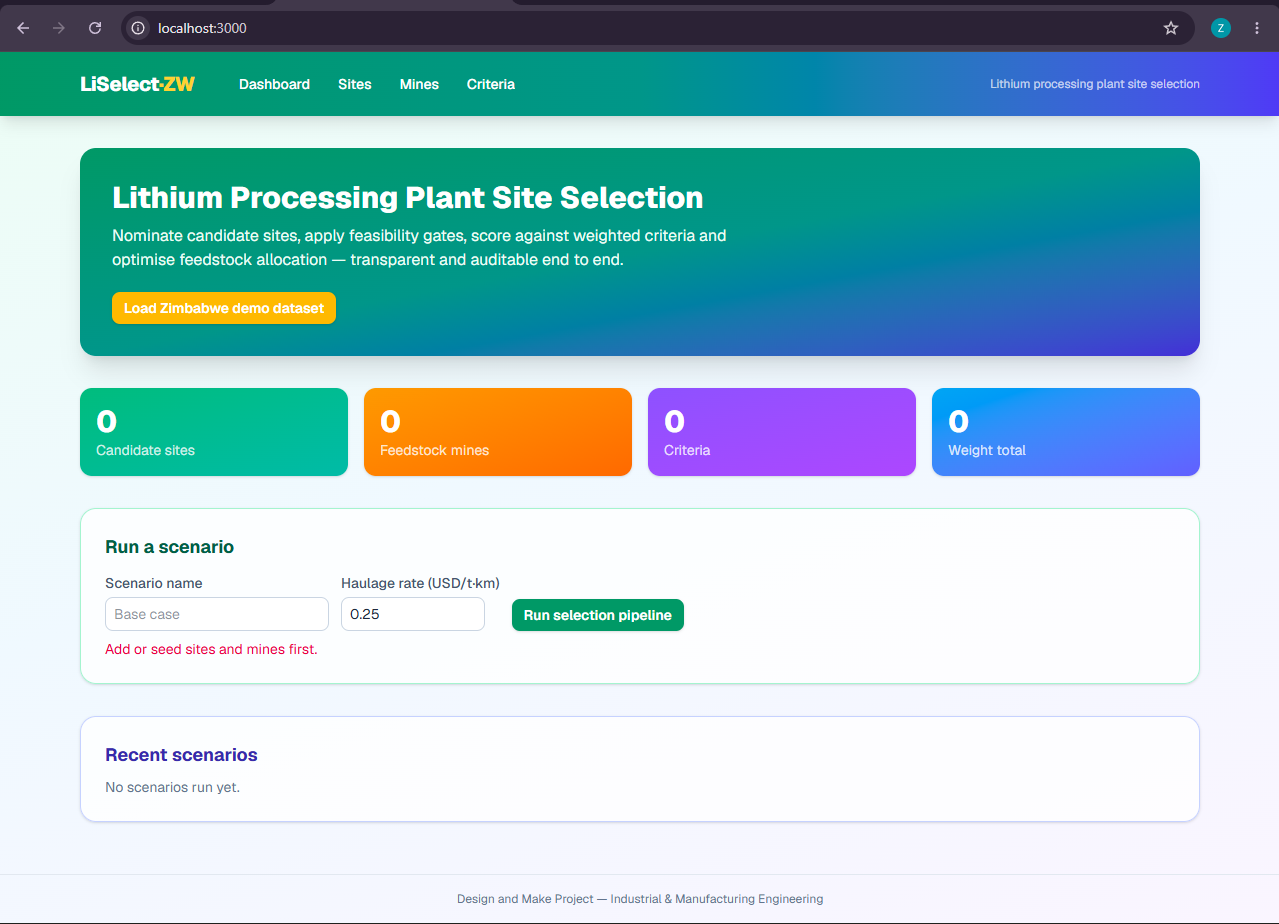
\includegraphics[width=0.85\textwidth]{home-page.png}
\caption{Dashboard with dataset summary and scenario launcher}
\label{fig:home}
\end{figure}

\subsection{Candidate sites}
The candidate sites page in Figure~\ref{fig:sites} lists each nominated
site with its capacity, water supply, grid reliability, settlement
distance, protected-land status and a live pass or fail indicator for
the site-only feasibility gates. The form beneath it collects the full
evidence set for a new site: location, capacity, utilities, logistics,
land, environmental indices, tailings suitability and fixed operating
cost. Every field is mandatory so that a site cannot be scored on a
silently assumed value, which implements the data-handling rule set out
in the methodology.

\begin{figure}[htbp]
\centering
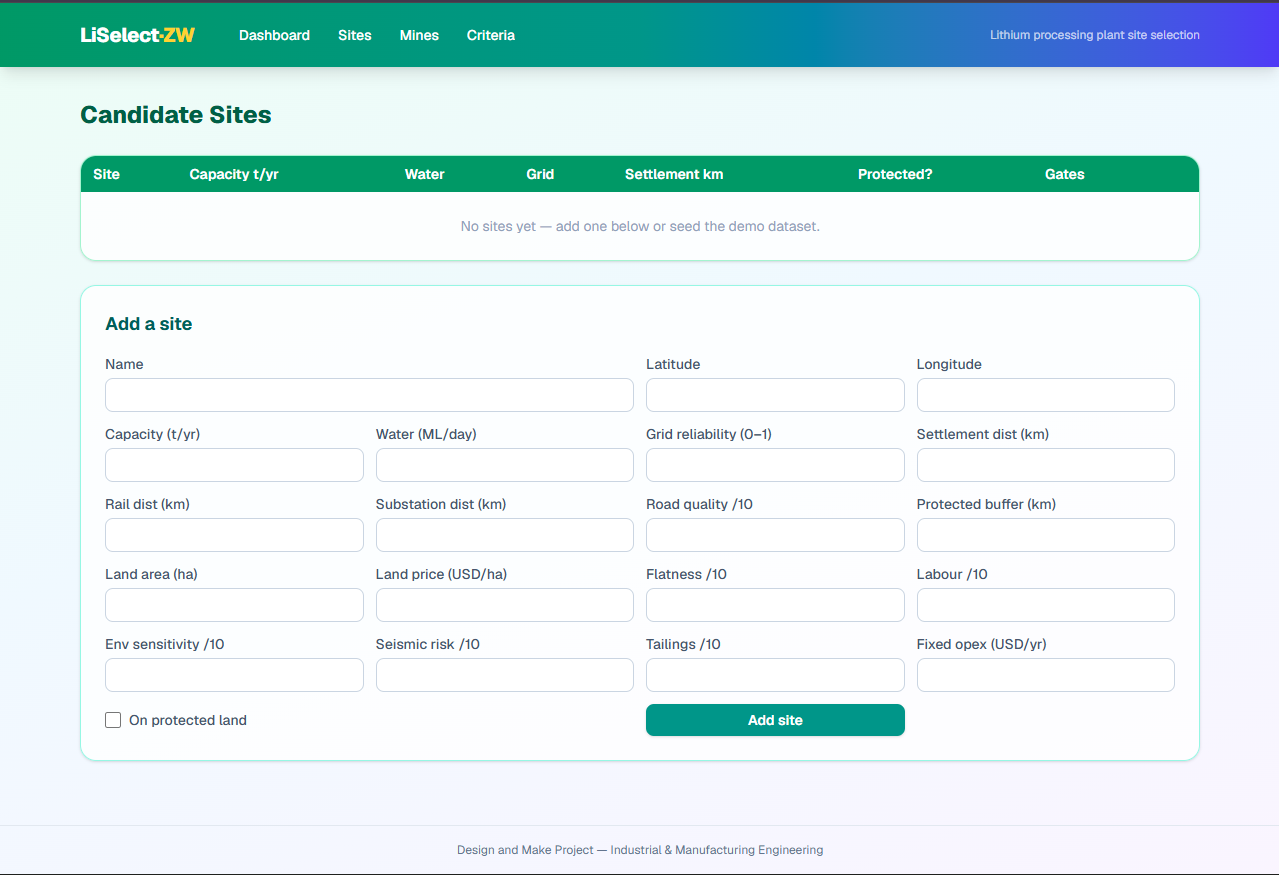
\includegraphics[width=0.85\textwidth]{sites-page.png}
\caption{Candidate sites page with the evidence entry form}
\label{fig:sites}
\end{figure}

\subsection{Feedstock mines}
Figure~\ref{fig:mines} shows the feedstock page. Each mine is entered
with its coordinates, annual supply limit and a descriptive note. The
supply limits drive both the allocation constraint and the feedstock
sufficiency gate, and the footer row reports total supply so the user
can see at a glance whether a plant of a given capacity can be fed.

\begin{figure}[htbp]
\centering
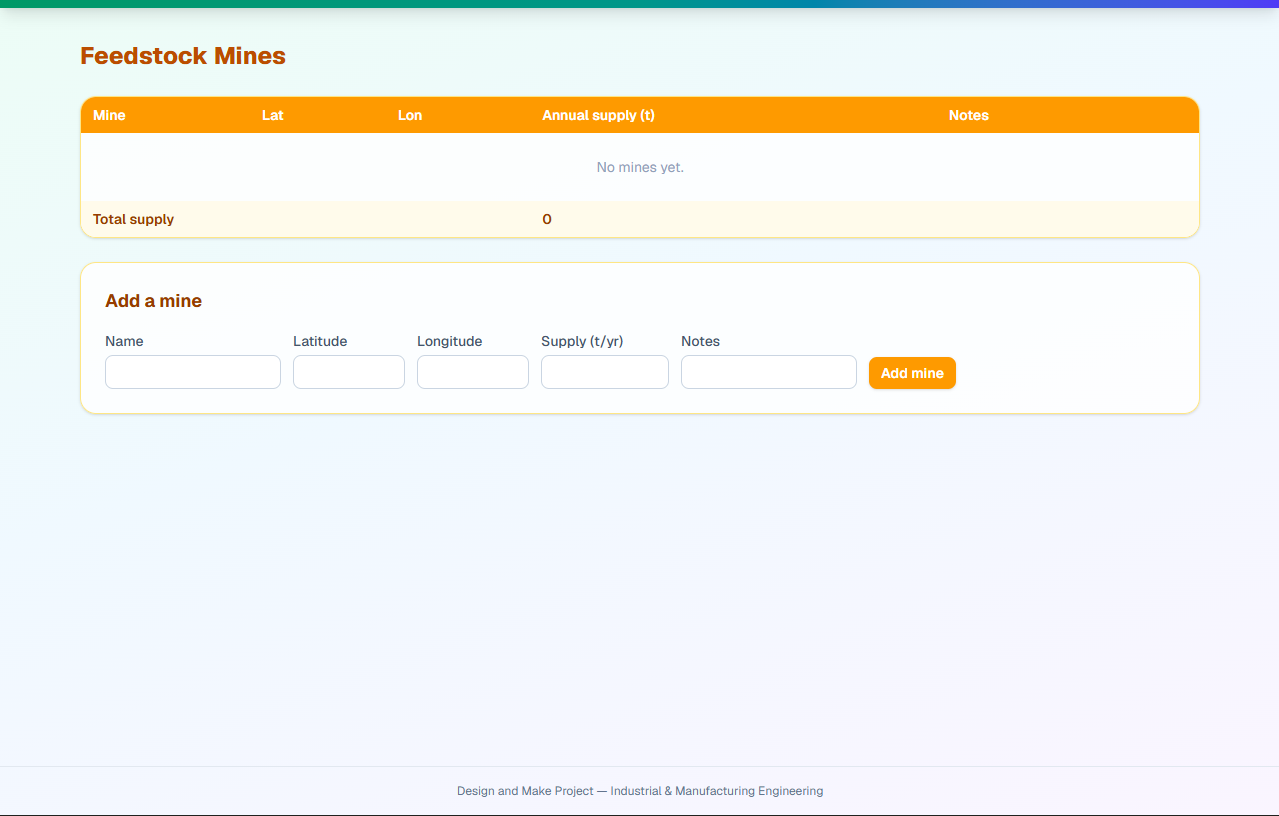
\includegraphics[width=0.85\textwidth]{feedstock-mines.png}
\caption{Feedstock mines page with total annual supply}
\label{fig:mines}
\end{figure}

\subsection{Criteria framework}
The criteria page in Figure~\ref{fig:criteria} is where the framework
is documented and the weights are set. Once the demonstration dataset
is loaded it lists the feasibility gates with their thresholds,
definitions and required evidence, followed by each criterion grouped
by factor group with its definition, evidence, source, direction,
normalisation range and an editable weight. The capture shown here
predates loading the dataset and therefore shows only the weight total
and the save control.

\begin{figure}[htbp]
\centering
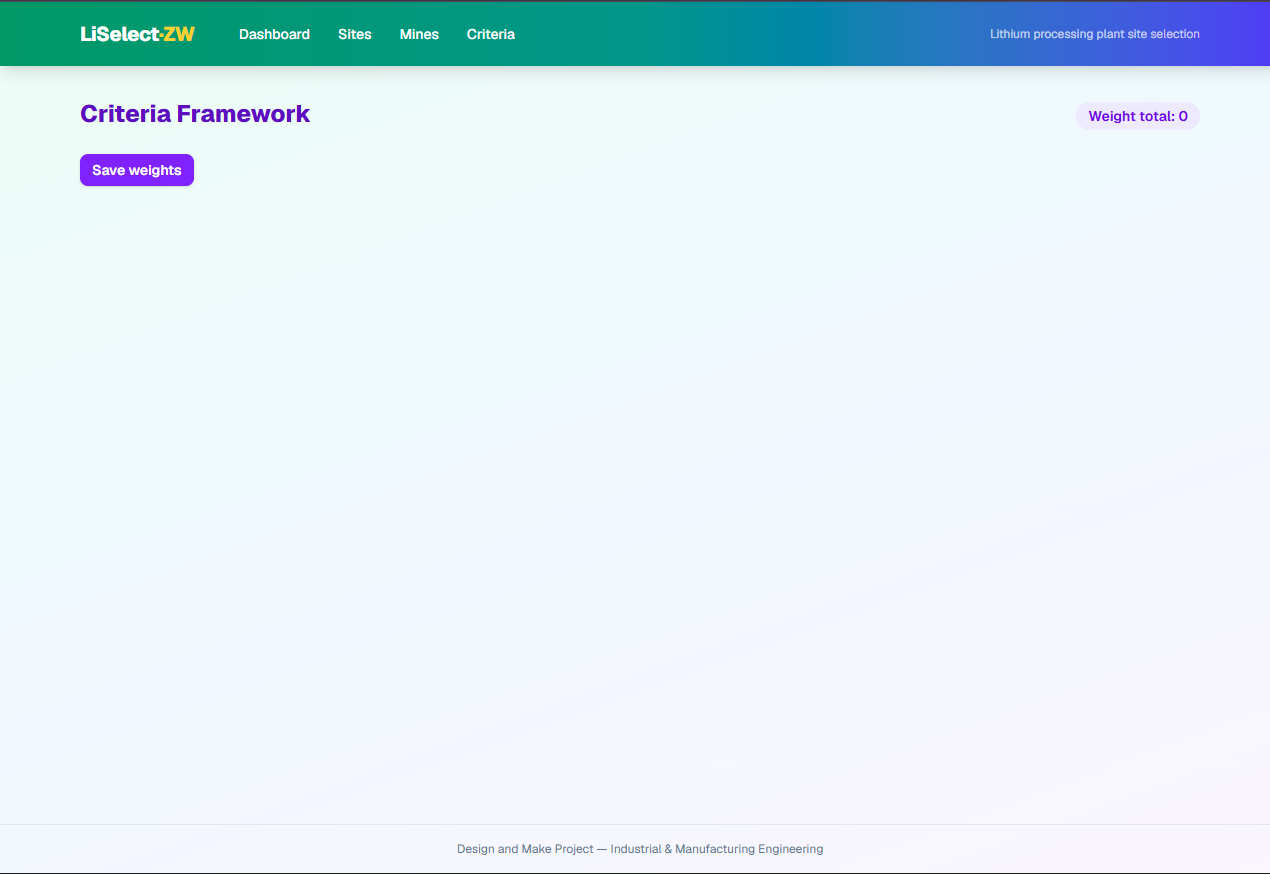
\includegraphics[width=0.85\textwidth]{criteria.png}
\caption{Criteria framework page before the dataset is loaded}
\label{fig:criteria}
\end{figure}

\section{Illustrative scenario}
Table 5.1 shows a worked example of the scored ranking stage for three
candidate sites after one site has already been eliminated at the
gates.

\begin{table}[h]
\centering
\caption{Illustrative scored output for surviving candidate sites}
\begin{tabular}{lccc}
\toprule
Factor group & Site A (Kwekwe) & Site B (Bikita) & Site C (Insiza) \\
\midrule
Industrial & 72 & 85 & 64 \\
Logistical & 80 & 58 & 71 \\
Utility & 66 & 74 & 55 \\
Land & 78 & 70 & 82 \\
Environmental & 84 & 62 & 77 \\
\midrule
\textbf{Composite} & \textbf{76.0} & \textbf{69.8} & \textbf{69.8} \\
\bottomrule
\end{tabular}
\end{table}

The numbers are illustrative rather than measured but they demonstrate
the shape of the output the system produces: a composite ranking that
decomposes into factor-group contributions which a stakeholder can
interrogate. In this example Site A wins on balanced strength rather
than dominance in any single group which is exactly the kind of result
informal judgement tends to miss.

\section{Results at the gate and allocation stages}
The gate stage of the illustrative scenario eliminated one of three
nominated sites on the settlement buffer gate. The surviving two plus
a third site brought the scored set to the three shown in Table 5.1.
The allocation stage produced a shipment pattern in which the two
nearest mines supply the bulk of plant capacity and the third mine
fills the remainder up to its supply limit which is the expected
signature of a cost-minimising transportation solution. Total annual
haulage cost emerges directly from the shipment table and the
sensitivity section reports that the ranking holds across the tested
perturbation ranges while the total cost moves modestly with unit
cost assumptions.

\section{Discussion of results}
The illustrative output shows the value of the decomposed report. Site
B is strongest on feedstock proximity and would win any informal
discussion anchored on ore tonnage. It loses the composite on
logistics and environmental grounds which is precisely the sort of
hidden weakness the system exists to expose. The sensitivity table
that accompanies the report tells the user whether the A-over-B margin
is stable under changed assumptions. In this illustration the margin
holds across the tested ranges so the recommendation is robust.

A second point from the illustration concerns the gate report. The
eliminated site does not simply disappear from the analysis. Its
failure reason is recorded and displayed which means a stakeholder
who favoured that site can see exactly why it fell out and can either
accept the reasoning or supply better evidence to overturn the gate
outcome. That is a materially different dynamic from informal
processes where a dismissed option leaves only resentment and no
record. The sensitivity output plays a complementary role. Where the
ranking is fragile under plausible perturbations the system says so
rather than presenting a brittle answer with false confidence. Both
behaviours flow from the same design commitment that the tool must
report uncertainty honestly rather than bury it.

\section{Wider implications}
Beyond the immediate application the work has two wider implications.
The first is that the architecture generalises. Nothing in the
pipeline is specific to lithium. The same gate-score-optimise
structure with a different criteria framework would serve the siting
of a gold plant, a cement works or a food processing facility. The
system is lithium-specific only in its criterion definitions which
are data rather than code. The second implication is methodological.
The project demonstrates that a defensible decision tool can be built
from well-understood parts without reaching for fashionable
techniques. The temptation in contemporary projects is to attach
machine learning to everything as a signal of modernity. This work
shows that an explicit algorithm chosen for its transparency is not a
compromise but a feature and that in decision support the boring
method is often the correct one.

\section{Limitations of the design}
Honest reporting requires stating what the design does not do. The
system evaluates the candidate sites it is given. It does not discover
sites and a user who nominates a weak candidate set will get the best
of a weak set. Distances are treated as user-entered values rather
than routed road-network distances which means the haulage costs in a
real deployment would be more accurate than the ones the current
design produces. The allocation model optimises a single objective,
cost, and does not trade cost against robustness or schedule. The
sensitivity ranges are stated perturbations rather than statistical
confidence intervals. None of these limitations is fatal to the
purpose of the tool but each defines a boundary the user should know.

\section{Implementation plan}
The design is sequenced so that the risky and foundational parts come
first and the decorative parts come last. The database schema and
input pages are built first since everything else depends on them.
The gate engine comes second because it is the simplest computation
and it establishes the pattern of persisted intermediate results. The
scoring engine follows, then the allocation solver, then the
sensitivity wrapper and the map last. The map is deliberately last
because it is the most visible feature and the least critical one and
putting it first is a classic way to end a project with a beautiful
map and no analysis behind it.

\begin{table}[h]
\centering
\caption{Implementation sequence and dependencies}
\begin{tabular}{clp{6.4cm}}
\toprule
Order & Component & Depends on \\
\midrule
1 & Database schema and input pages & Nothing \\
2 & Gate engine & Schema and inputs \\
3 & Scoring engine & Gates \\
4 & Allocation solver & Schema, mines \\
5 & Sensitivity wrapper & Full pipeline \\
6 & Map layer & Sites and mines data \\
\bottomrule
\end{tabular}
\end{table}

\section{Contribution of the work}
The contribution of the project is threefold. At the practical level
it delivers a fully specified design for a tool that does not
currently exist in the Zimbabwean lithium context. At the
methodological level it shows how three established techniques,
feasibility gating, weighted scoring and allocation optimisation, can
be packaged into one auditable pipeline rather than left as separate
textbook topics. At the educational level it demonstrates a complete
concept development exercise in which alternatives were genuinely
generated, fairly evaluated and honestly rejected with reasons rather
than token alternatives erected to make a pre-chosen answer look
considered. The last point matters more than it might appear. Concept
development exercises often degenerate into theatre where one concept
is the real answer and the others are straw men. Every rejected
concept in this report was a legitimate approach that would be the
right choice under different project circumstances and each was
rejected for stated reasons rather than by construction.

It is also worth stating plainly what the project does not claim. The
worked scenario in Table 5.1 uses illustrative numbers and the system
described is a design rather than a finished deployed artefact. The
claim being made is that the design is sound, complete and implementable
as specified not that a deployed instance has already processed real
site data. That distinction matters for honest assessment of the work
and it is stated so the contribution is judged on what it actually is.

\section{Recommendations}
Future work should connect the system to real spatial datasets so gate
checks like protected-area overlap and settlement buffers are computed
from geometry rather than user assertions. Adding a second plant to
the allocation model would extend the tool from siting to regional
planning. A formal AHP module for deriving weights from stakeholder
pairwise comparisons, as sketched in Concept 4, would strengthen the
weighting step and give the weights a documented provenance rather
than relying on judgement. Longer term, integration with a genuine
road-network distance service would replace straight-line or
user-entered distances with routed ones and connecting the tool to the
geological survey would let candidate sites be nominated from deposit
data rather than declared by hand.

A practical recommendation for the student continuation of this
project is to build the system incrementally: database and input pages
first, gate engine second, scoring third, allocation fourth and the
map last. The map is the most visible feature and the least critical
one which makes it a poor place to start.

\section{Suggestions for future research}
Beyond the implementation recommendations above, the project suggests
three directions for future research. The first is empirical
validation. Once the system is implemented and run against real
candidate sites the rankings it produces should be compared against
the judgement of experienced practitioners to see where they agree
and where the structured process surfaces something intuition missed.
The second is weight derivation. The current design accepts weights
as user inputs and the integration of a formal AHP module would give
those weights a documented provenance. The third is extension to the
multi-plant case. Zimbabwe's beneficiation programme will eventually
face the question of how many plants and where and the general
formulation already written for the allocation model accommodates that
extension directly.

\section{Conclusion}
The project set out to design a site selection system for a lithium
processing plant in Zimbabwe. The delivered design combines a
structured criteria framework, feasibility gates, weighted scoring and
a transparent allocation optimisation inside a single web application.
Five candidate concepts were evaluated and the Next.js, SQLite/Prisma
and OpenStreetMap architecture was selected. The result is a system
whose recommendations are repeatable, explainable and defensible and
whose design is fully specified for implementation.

Returning to the research questions posed in Chapter 1, the design
answers each of them. The criteria that most strongly determine
suitability are utility and logistical factors which is why the
framework weights them accordingly. Feasibility gates and weighted
scoring combine cleanly provided gates run first and failures are
never allowed to be compensated by scores. Facility selection and
feedstock allocation model as a transportation linear program whose
constraints correspond one to one with physical limits. Sensitivity
is communicated by perturbation ranges with fragile recommendations
flagged explicitly. The work is complete in the sense that every
objective has a corresponding designed mechanism and open in the
sense that implementation and empirical validation remain for future
work as the recommendations state.

% ============================ REFERENCES ============================
\begin{thebibliography}{99}
\addcontentsline{toc}{chapter}{REFERENCES}

\bibitem[Belton and Stewart(2002)]{belton}
Belton, V. and Stewart, T.J. (2002) \textit{Multiple Criteria Decision
Analysis: An Integrated Approach}. Boston: Kluwer Academic.

\bibitem[Chikodzi(2023)]{chikodzi}
Chikodzi, D. (2023) `Lithium mining and beneficiation prospects in
Zimbabwe', \textit{African Journal of Science, Technology, Innovation
and Development}, 15(4), pp. 512--524.

\bibitem[Choudhary and Shankar(2012)]{choudhary}
Choudhary, D. and Shankar, R. (2012) `An STEEP-fuzzy AHP-TOPSIS
framework for evaluation and selection of thermal power plant
location', \textit{Energy}, 42(1), pp. 510--521.

\bibitem[Daskin(2013)]{daskin}
Daskin, M.S. (2013) \textit{Network and Discrete Location: Models,
Algorithms, and Applications}. 2nd edn. Hoboken: Wiley.

\bibitem[Eiselt and Marianov(2011)]{eiselt}
Eiselt, H.A. and Marianov, V. (eds.) (2011) \textit{Foundations of
Location Analysis}. New York: Springer.

\bibitem[FAO(2017)]{fao}
Food and Agriculture Organization (2017) \textit{Water for Sustainable
Food and Agriculture}. Rome: FAO.

\bibitem[Flexer et al.(2018)]{flexer}
Flexer, V., Baspineiro, C.F. and Galli, C.I. (2018) `Lithium recovery
from brines: a vital raw material for green energies with a potential
environmental impact', \textit{Science of the Total Environment}, 639,
pp. 1188--1204.

\bibitem[Haklay and Weber(2008)]{haklay}
Haklay, M. and Weber, P. (2008) `OpenStreetMap: user-generated street
maps', \textit{IEEE Pervasive Computing}, 7(4), pp. 12--18.

\bibitem[Koech and Langat(2018)]{koech}
Koech, R. and Langat, P. (2018) `Improving irrigation water use
efficiency: a review', \textit{International Journal of Environmental
Science}, 3(1), pp. 1--19.

\bibitem[Malczewski(2004)]{malczewski}
Malczewski, J. (2004) `GIS-based land-use suitability analysis: a
critical overview', \textit{Progress in Planning}, 62(1), pp. 3--65.

\bibitem[Mukono(2023)]{mukono}
Mukono, T. (2023) `Zimbabwe's lithium export ban and the push for
local beneficiation', \textit{Journal of Southern African Studies},
49(2), pp. 301--318.

\bibitem[Musingwini and Minnitt(2008)]{musingwini}
Musingwini, C. and Minnitt, R.C.A. (2008) `Ranked factor-based
selection of mining projects', \textit{Journal of the Southern African
Institute of Mining and Metallurgy}, 108(1), pp. 37--44.

\bibitem[Pham et al.(2019)]{pham}
Pham, B.T. et al. (2019) `A novel machine learning approach for land
susceptibility mapping', \textit{Geoscience Frontiers}, 10(4), pp.
1341--1354.

\bibitem[Rezaei(2015)]{rezaei}
Rezaei, J. (2015) `Best-worst multi-criteria decision-making method',
\textit{Omega}, 53, pp. 49--57.

\bibitem[Saaty(1980)]{saaty}
Saaty, T.L. (1980) \textit{The Analytic Hierarchy Process}. New York:
McGraw-Hill.

\bibitem[Shim et al.(2002)]{shim}
Shim, J.P. et al. (2002) `Past, present and future of decision support
technology', \textit{Decision Support Systems}, 33(2), pp. 111--126.

\bibitem[Store and Kangas(2001)]{store}
Store, R. and Kangas, J. (2001) `Integrating spatial multi-criteria
evaluation and expert knowledge for GIS-based habitat suitability
modelling', \textit{Landscape and Urban Planning}, 55(2), pp. 79--93.

\bibitem[Tavana et al.(2017)]{tavana}
Tavana, M. et al. (2017) `A hybrid MCDM model for mining project
selection', \textit{Resources Policy}, 52, pp. 220--234.

\bibitem[Turskis and Zavadskas(2010)]{turskis}
Turskis, Z. and Zavadskas, E.K. (2010) `A novel method for multiple
criteria analysis: grey additive ratio assessment',
\textit{Technological and Economic Development of Economy}, 16(4), pp.
650--662.

\bibitem[Weber(1909)]{weber}
Weber, A. (1909) \textit{Theory of the Location of Industries}.
Chicago: University of Chicago Press.

\end{thebibliography}

% ============================ APPENDICES ============================
\appendix

\chapter{DATABASE SCHEMA}
The application stores its data in a single SQLite file accessed through
the Prisma ORM. Listing~\ref{lst:schema} reproduces the schema file.
\texttt{Mine} and \texttt{Site} hold the user-entered evidence,
\texttt{Criterion} holds the criteria framework with its definition,
evidence requirement, source, normalisation range and weight, and
\texttt{Scenario} stores each saved run as a JSON result so that a
scenario cannot be silently revised after the fact.

\lstinputlisting[language=Prisma,caption={Prisma database schema (\texttt{prisma/schema.prisma})},label={lst:schema}]{../../prisma/schema.prisma}

\chapter{BUSINESS LOGIC SOURCE CODE}
This appendix reproduces the core of the decision pipeline. The code is
included directly from the project source so that it matches the
implemented system. The order follows the pipeline: gates, scoring,
allocation, cost, cost-optimal selection and sensitivity.

\section{Feasibility gates}
Each gate is a named hard constraint with a threshold, a definition and
the evidence required. The supply sufficiency gate is evaluated only when
the mines are known, and a site that fails any gate is excluded.

\lstinputlisting[language=TypeScript,firstline=1,lastline=35,caption={Gate definitions (first gates), \texttt{lib/gates.ts}},label={lst:gates1}]{../../lib/gates.ts}

\lstinputlisting[language=TypeScript,firstline=83,firstnumber=83,lastline=108,caption={Supply sufficiency gate and gate evaluation, \texttt{lib/gates.ts}},label={lst:gates2}]{../../lib/gates.ts}

\section{Normalisation and weighted scoring}
Each measurement is scaled to a 0--100 value using the criterion range,
inverted for cost-type criteria, and combined using weights that are
normalised by their sum.

\lstinputlisting[language=TypeScript,firstline=1,lastline=52,caption={Evidence values, normalisation and scoring, \texttt{lib/scoring.ts}},label={lst:scoring}]{../../lib/scoring.ts}

\section{Feedstock allocation}
For a single plant the transportation problem is solved exactly by
shipping from the nearest mines first until the plant capacity is met or
the supply is exhausted.

\lstinputlisting[language=TypeScript,firstline=20,firstnumber=20,lastline=56,caption={Allocation of mine supply to a plant, \texttt{lib/transport.ts}},label={lst:transport}]{../../lib/transport.ts}

\section{Annual cost model}
\lstinputlisting[language=TypeScript,caption={Annual cost model, \texttt{lib/cost.ts}},label={lst:cost}]{../../lib/cost.ts}

\section{Cost-optimal facility selection}
Every site that passes all gates is scored, allocated and priced. The
site with the lowest annual cost is the optimiser's choice and the
highest-scoring site is reported alongside it.

\lstinputlisting[language=TypeScript,firstline=33,firstnumber=33,lastline=66,caption={Facility selection and allocation, \texttt{lib/evaluate.ts}},label={lst:evaluate}]{../../lib/evaluate.ts}

\section{Sensitivity analysis}
The pipeline is re-run under perturbed haulage rates, mine supply limits
and criterion weights. A recommendation that changes under any tested
perturbation is flagged as fragile.

\lstinputlisting[language=TypeScript,firstline=40,firstnumber=40,lastline=96,caption={Sensitivity analysis, \texttt{lib/sensitivity.ts}},label={lst:sensitivity}]{../../lib/sensitivity.ts}

\end{document}
